\chapter{Results}
\label{chap:results}

\section{Frontend showcase}
\label{sec:frontend-showcase}

This section showcases the resulting frontend application, which serves as the primary interface for the Roskilde Festival safety team to access and analyze crowd dynamics data. The interface is designed to be intuitive, presenting complex data through interactive charts and maps. The following figures illustrate the key features and functionalities of the application. Note that data shown from June 30th to July 2nd corresponds to the Eos stage, while data from July 3rd onwards corresponds to the Arena stage.

Following Eric Ries' Build-Measure-Learn feedback loop, the application was developed iteratively, with each version being refined based on user feedback. The loop started with a long Learn phase, where many conversations were held with the safety team to really grasp their needs and workflows. The product's first version was then built (Build), and Roskilde Festival's Mads and Morten Therkildsen were subsequently invited to provide feedback. Feedback in this case is the qualitative data netted from the Measure phase. This feedback was then analyzed and used to refine the product, which was then again presented and evaluated. The process was repeated until the final version was reached, which was presented in the workshop outlined in Section \ref{sec:business-value}.

The resulting frontend application directly addresses the requirement specifications outlined in Section \ref{sec:objectives}. Core metric extraction (Requirement 1) is achieved through the backend processing pipeline (detailed in Chapter 3), with the frontend serving as the access point for these metrics. Figures \ref{fig:showcase:dashboard} through \ref{fig:showcase:concerts} demonstrate the visualization of key metrics such as cumulative totals, ingress/egress flow rates, and concert-specific flow analyses, with movement patterns and crowd density heatmaps visualized in Figures \ref{fig:showcase:map-movement} and \ref{fig:showcase:map-density}, respectively. The platform provides an intuitive user interface (Requirement 2), by including interactivity through filtering (Figure \ref{fig:showcase:filter}), and visualization tooltips (Figure \ref{fig:showcase:flow-total}), ensuring users can easily filter and understand the presented data. Regarding compliant data handling (Requirement 3), the system architecture is designed for compliance with data protection regulations (Section \ref{sec:legal-feasibility}). Importantly, immediately following the inputting of video footage into the object detection model (Section \ref{sec:cv_model}), no biometric data is stored. The images are converted into quantitative data as well as anonymous geographic position data. This ensures that all historical data retained is fully anonymized, thereby protecting privacy while still providing valuable insights.


\begin{figure}[H]
  \centering
  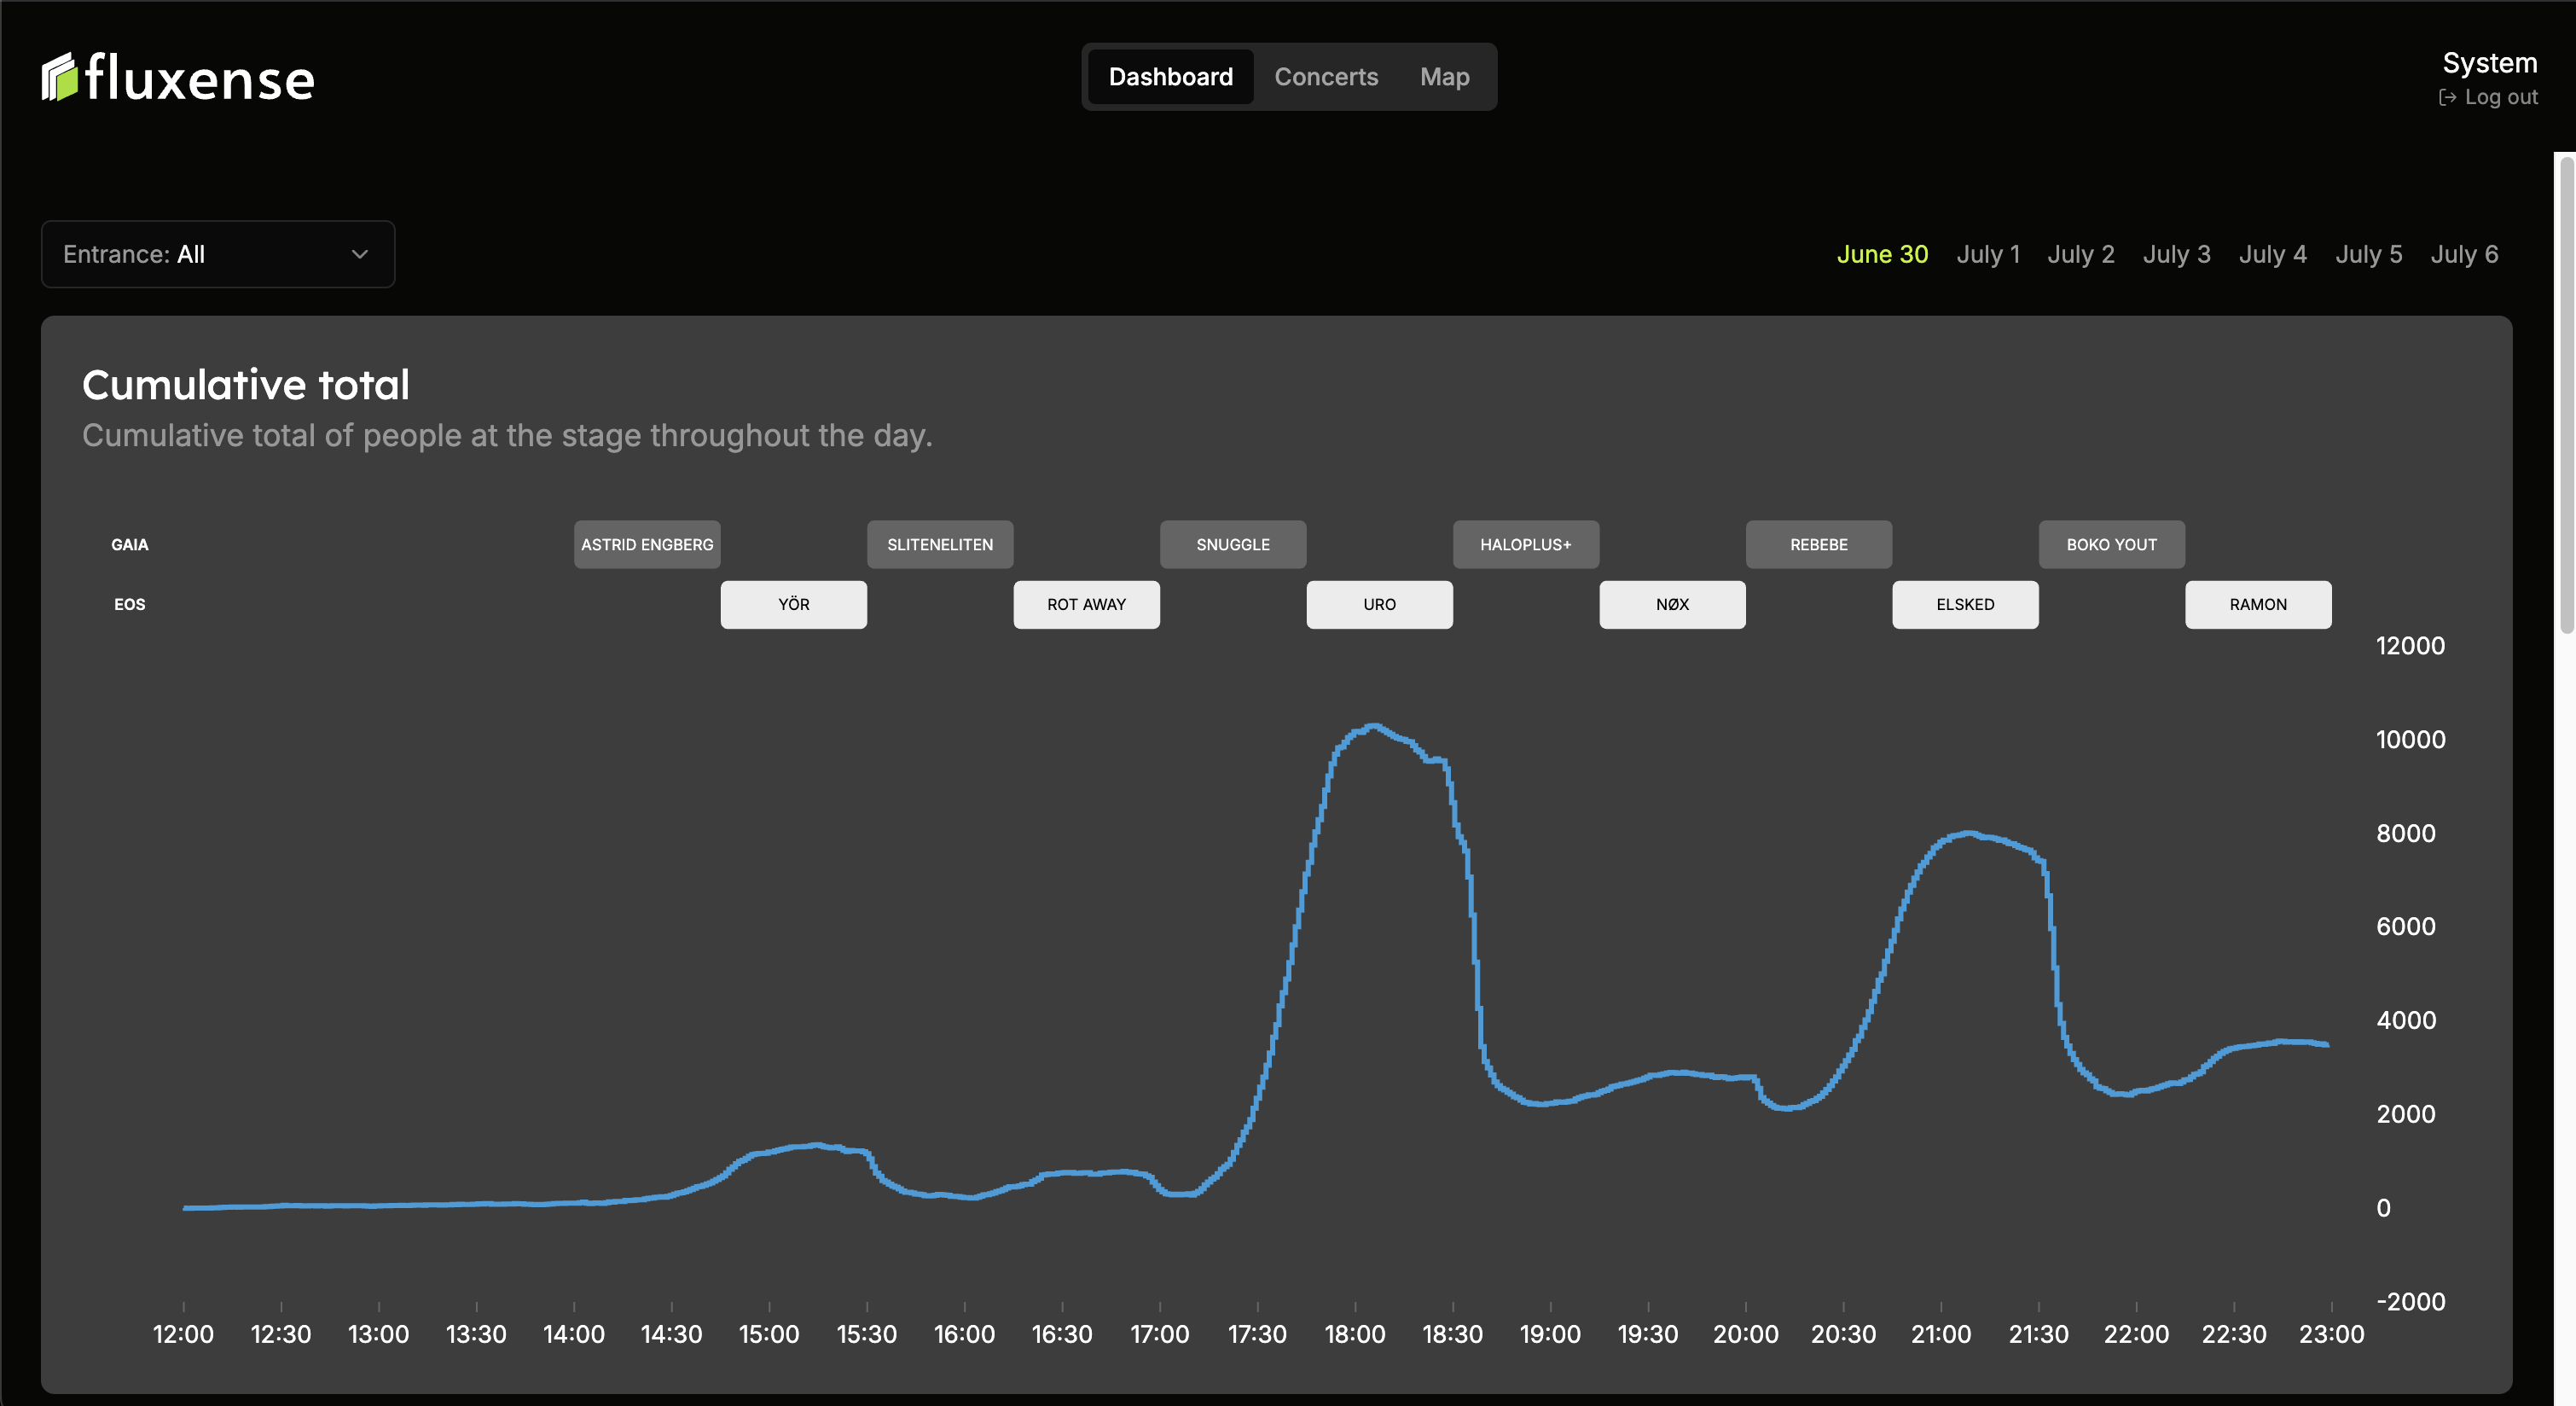
\includegraphics[width=\textwidth]{Pictures/Misc/Frontend/cum_total.png}
  \caption{The 'Dashboard' view displaying the cumulative total number of people estimated to be at the selected stage (Eos or Arena) throughout the day. An overlay along the top indicates the scheduled concert timings for the observed stage. Based on feedback requesting analysis of inter-stage flow (Appendix \ref{appendix:rf-sep-24}), schedules for adjacent stages (i.e., Gaia when observing Eos, or Orange stage when observing Arena) were also included.}
  \label{fig:showcase:dashboard}

\end{figure}


\begin{figure}[H]
  \centering
  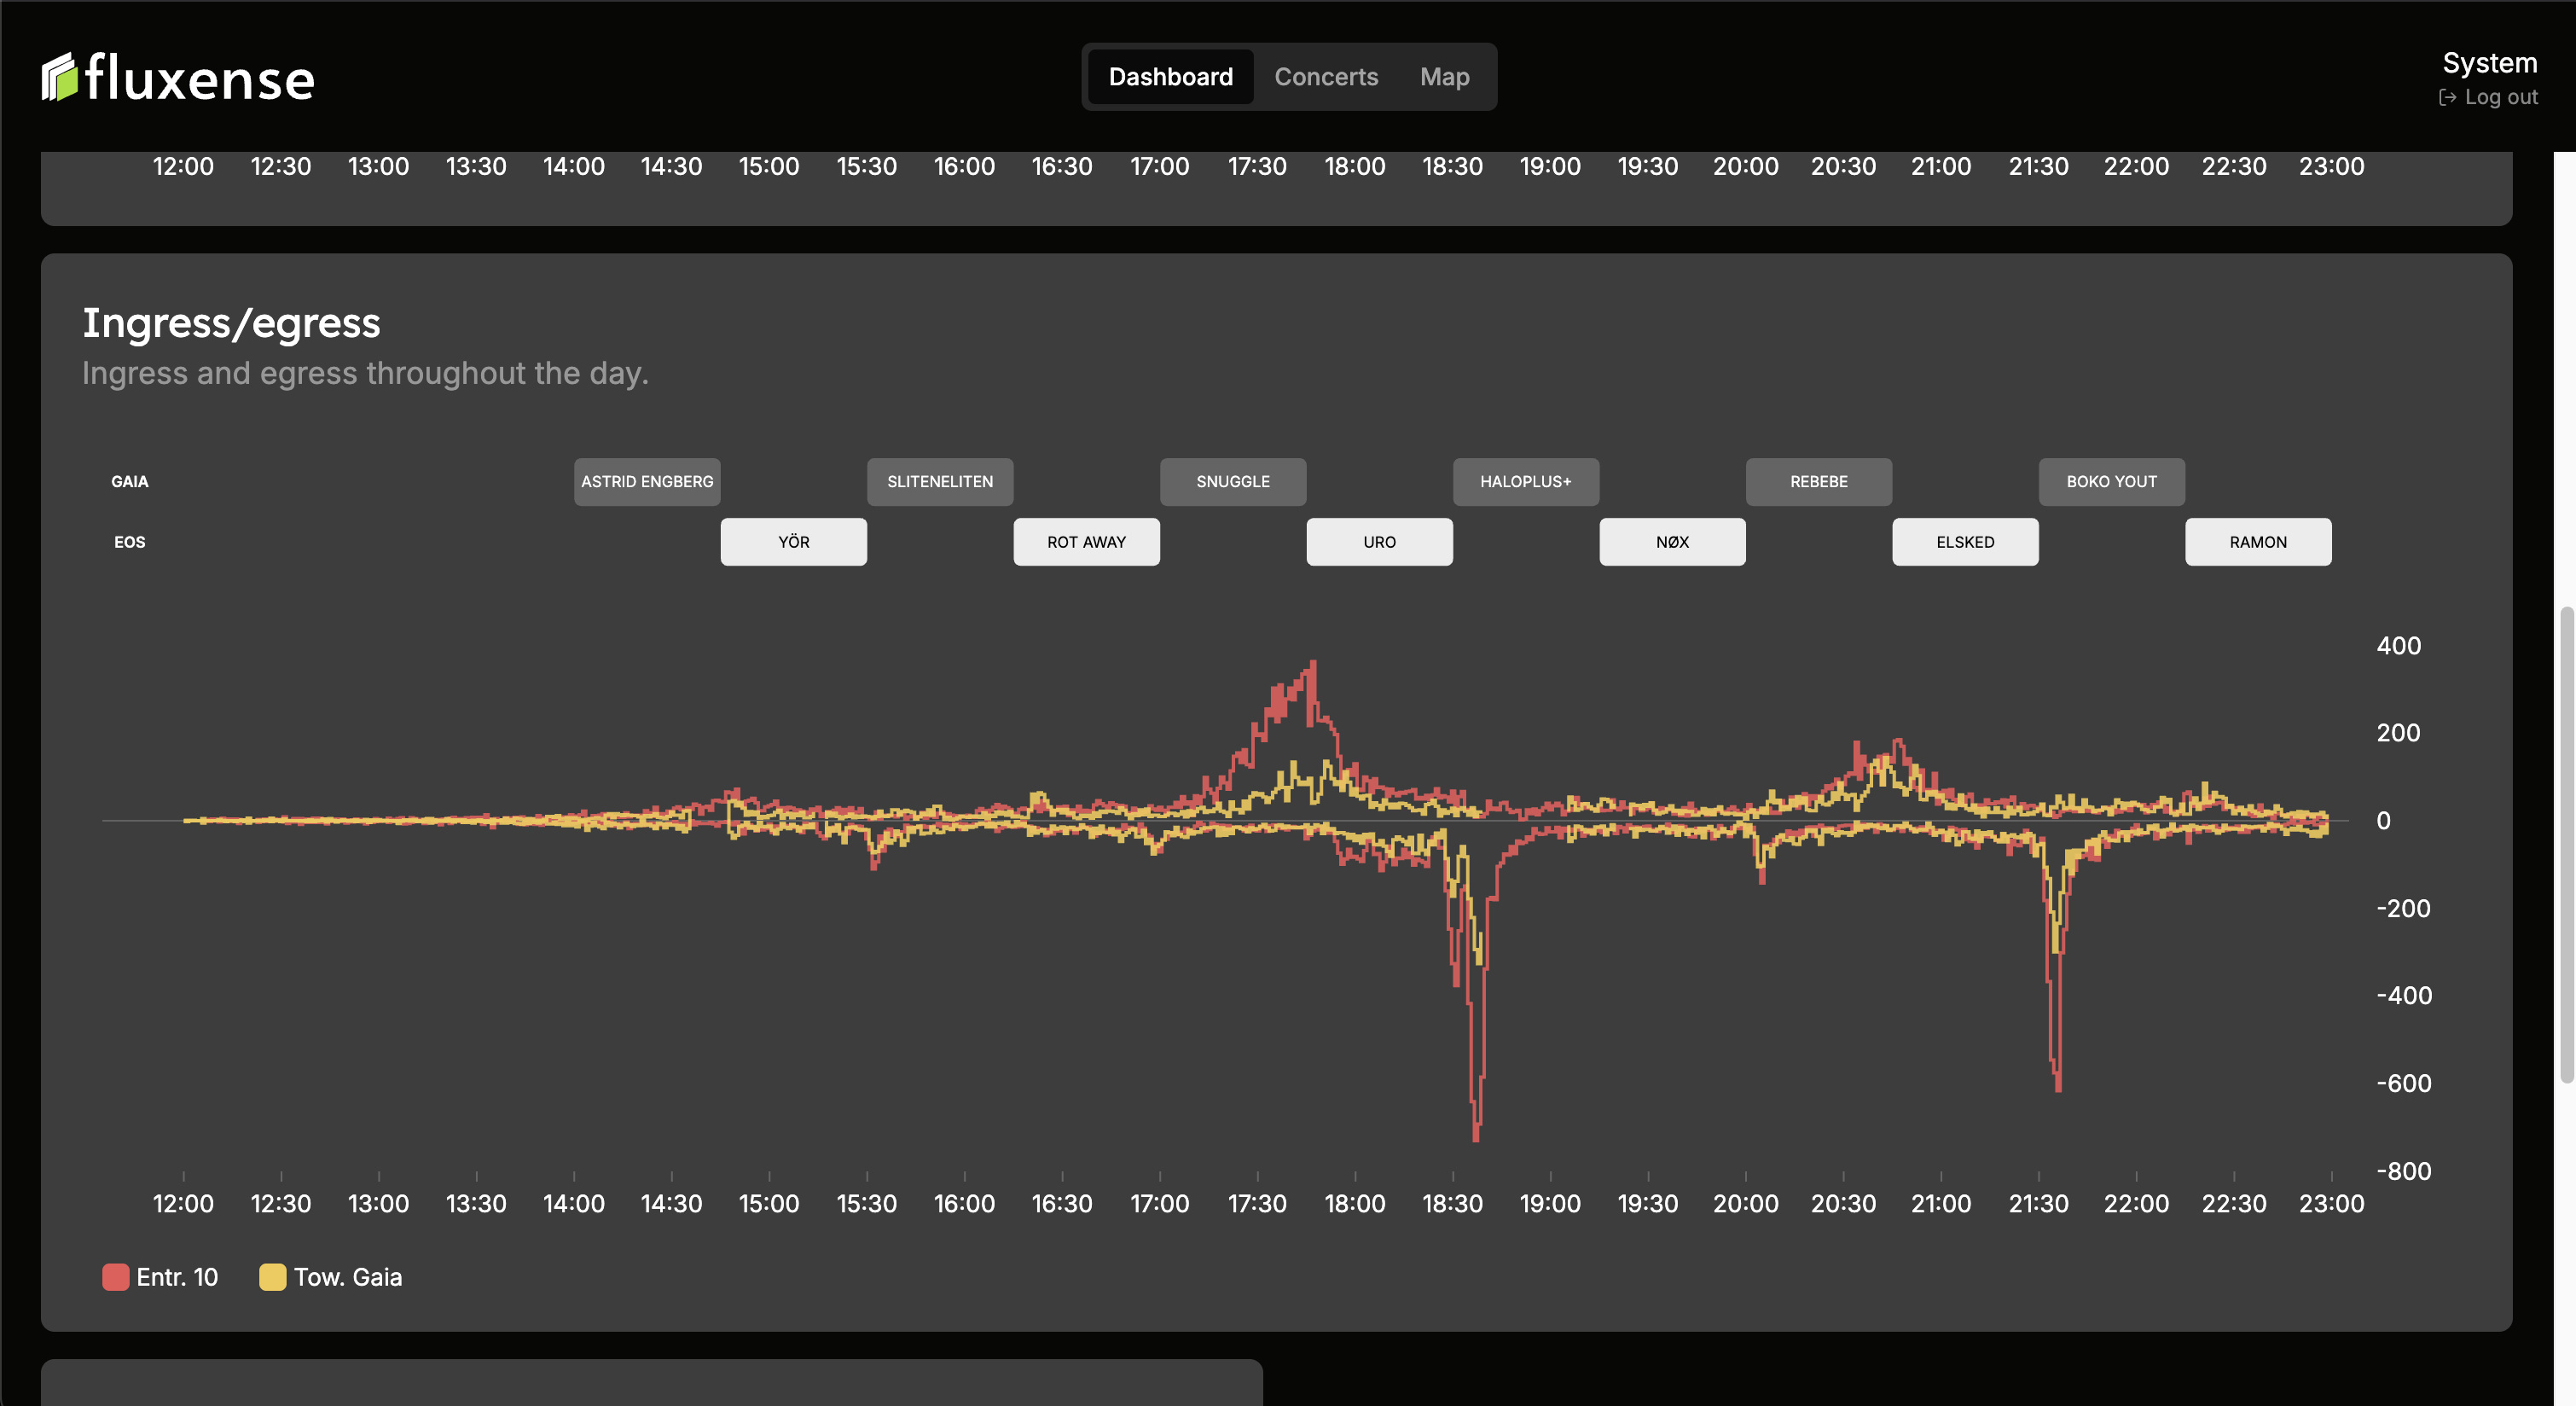
\includegraphics[width=\textwidth]{Pictures/Misc/Frontend/ingress_egress.png}
  \caption{The 'Dashboard' view showing the ingress (positive values) and egress (negative values) rates in people per minute throughout the day. Displaying data split by individual entrances (e.g., "Entr. 10", "Tow. Gaia") was implemented based on feedback requesting insight into the load of each entrance. The concert schedule overlay, including schedules from relevant adjacent stages added per user feedback, is also present for context.}
  \label{fig:showcase:ingress-egress}

\end{figure}


\begin{figure}[H]
  \centering
  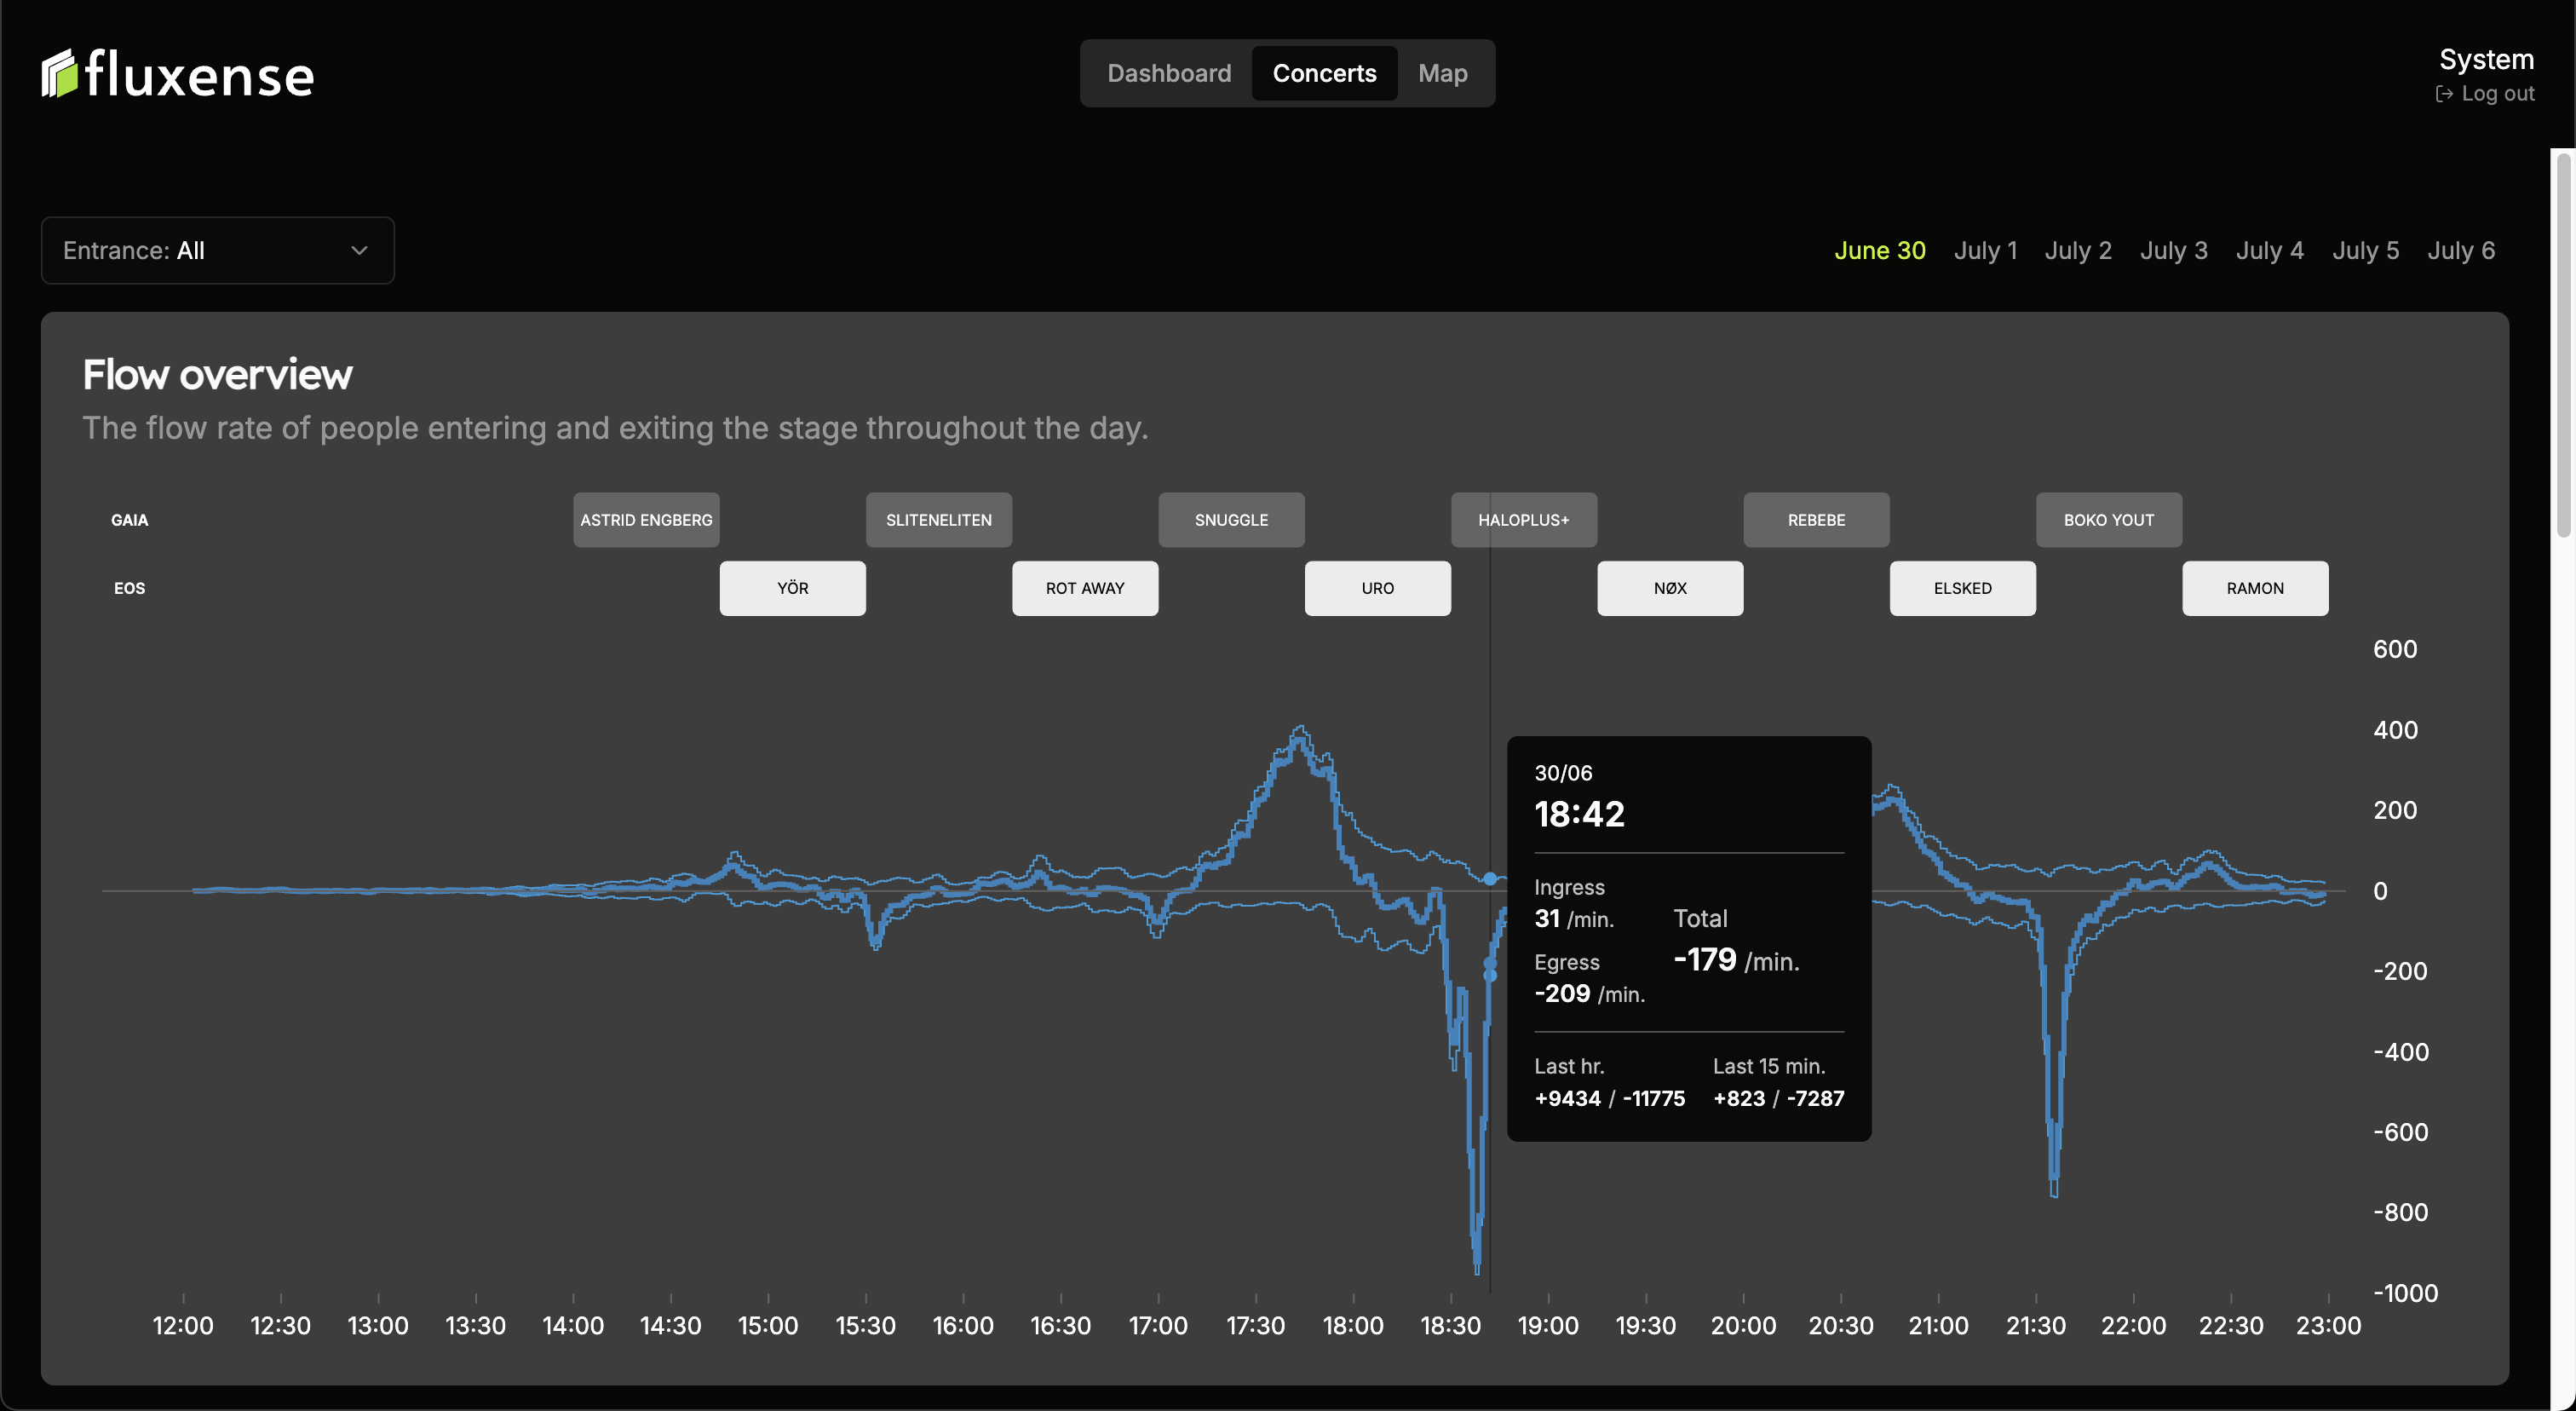
\includegraphics[width=\textwidth]{Pictures/Misc/Frontend/flow_total.png}
  \caption{The 'Concerts' view presenting the overall flow rates. It displays ingress-flow (top line), egress-flow (bottom line), and the total flow (bold middle line). Based on feedback, flow rates are presented in people per minute for easier interpretation compared to the initial people/second unit (Appendix \ref{appendix:rf-feb-25}). Hovering over the chart reveals a tooltip displaying instantaneous ingress, egress, and total flow rates at a given minute, along with aggregated ingress/egress totals over the last 15 and 60 minutes, aligning with RF's requested analysis intervals. The concert schedule overlay is also present for context.}
  \label{fig:showcase:flow-total}

\end{figure}

\begin{figure}[H]
  \centering
  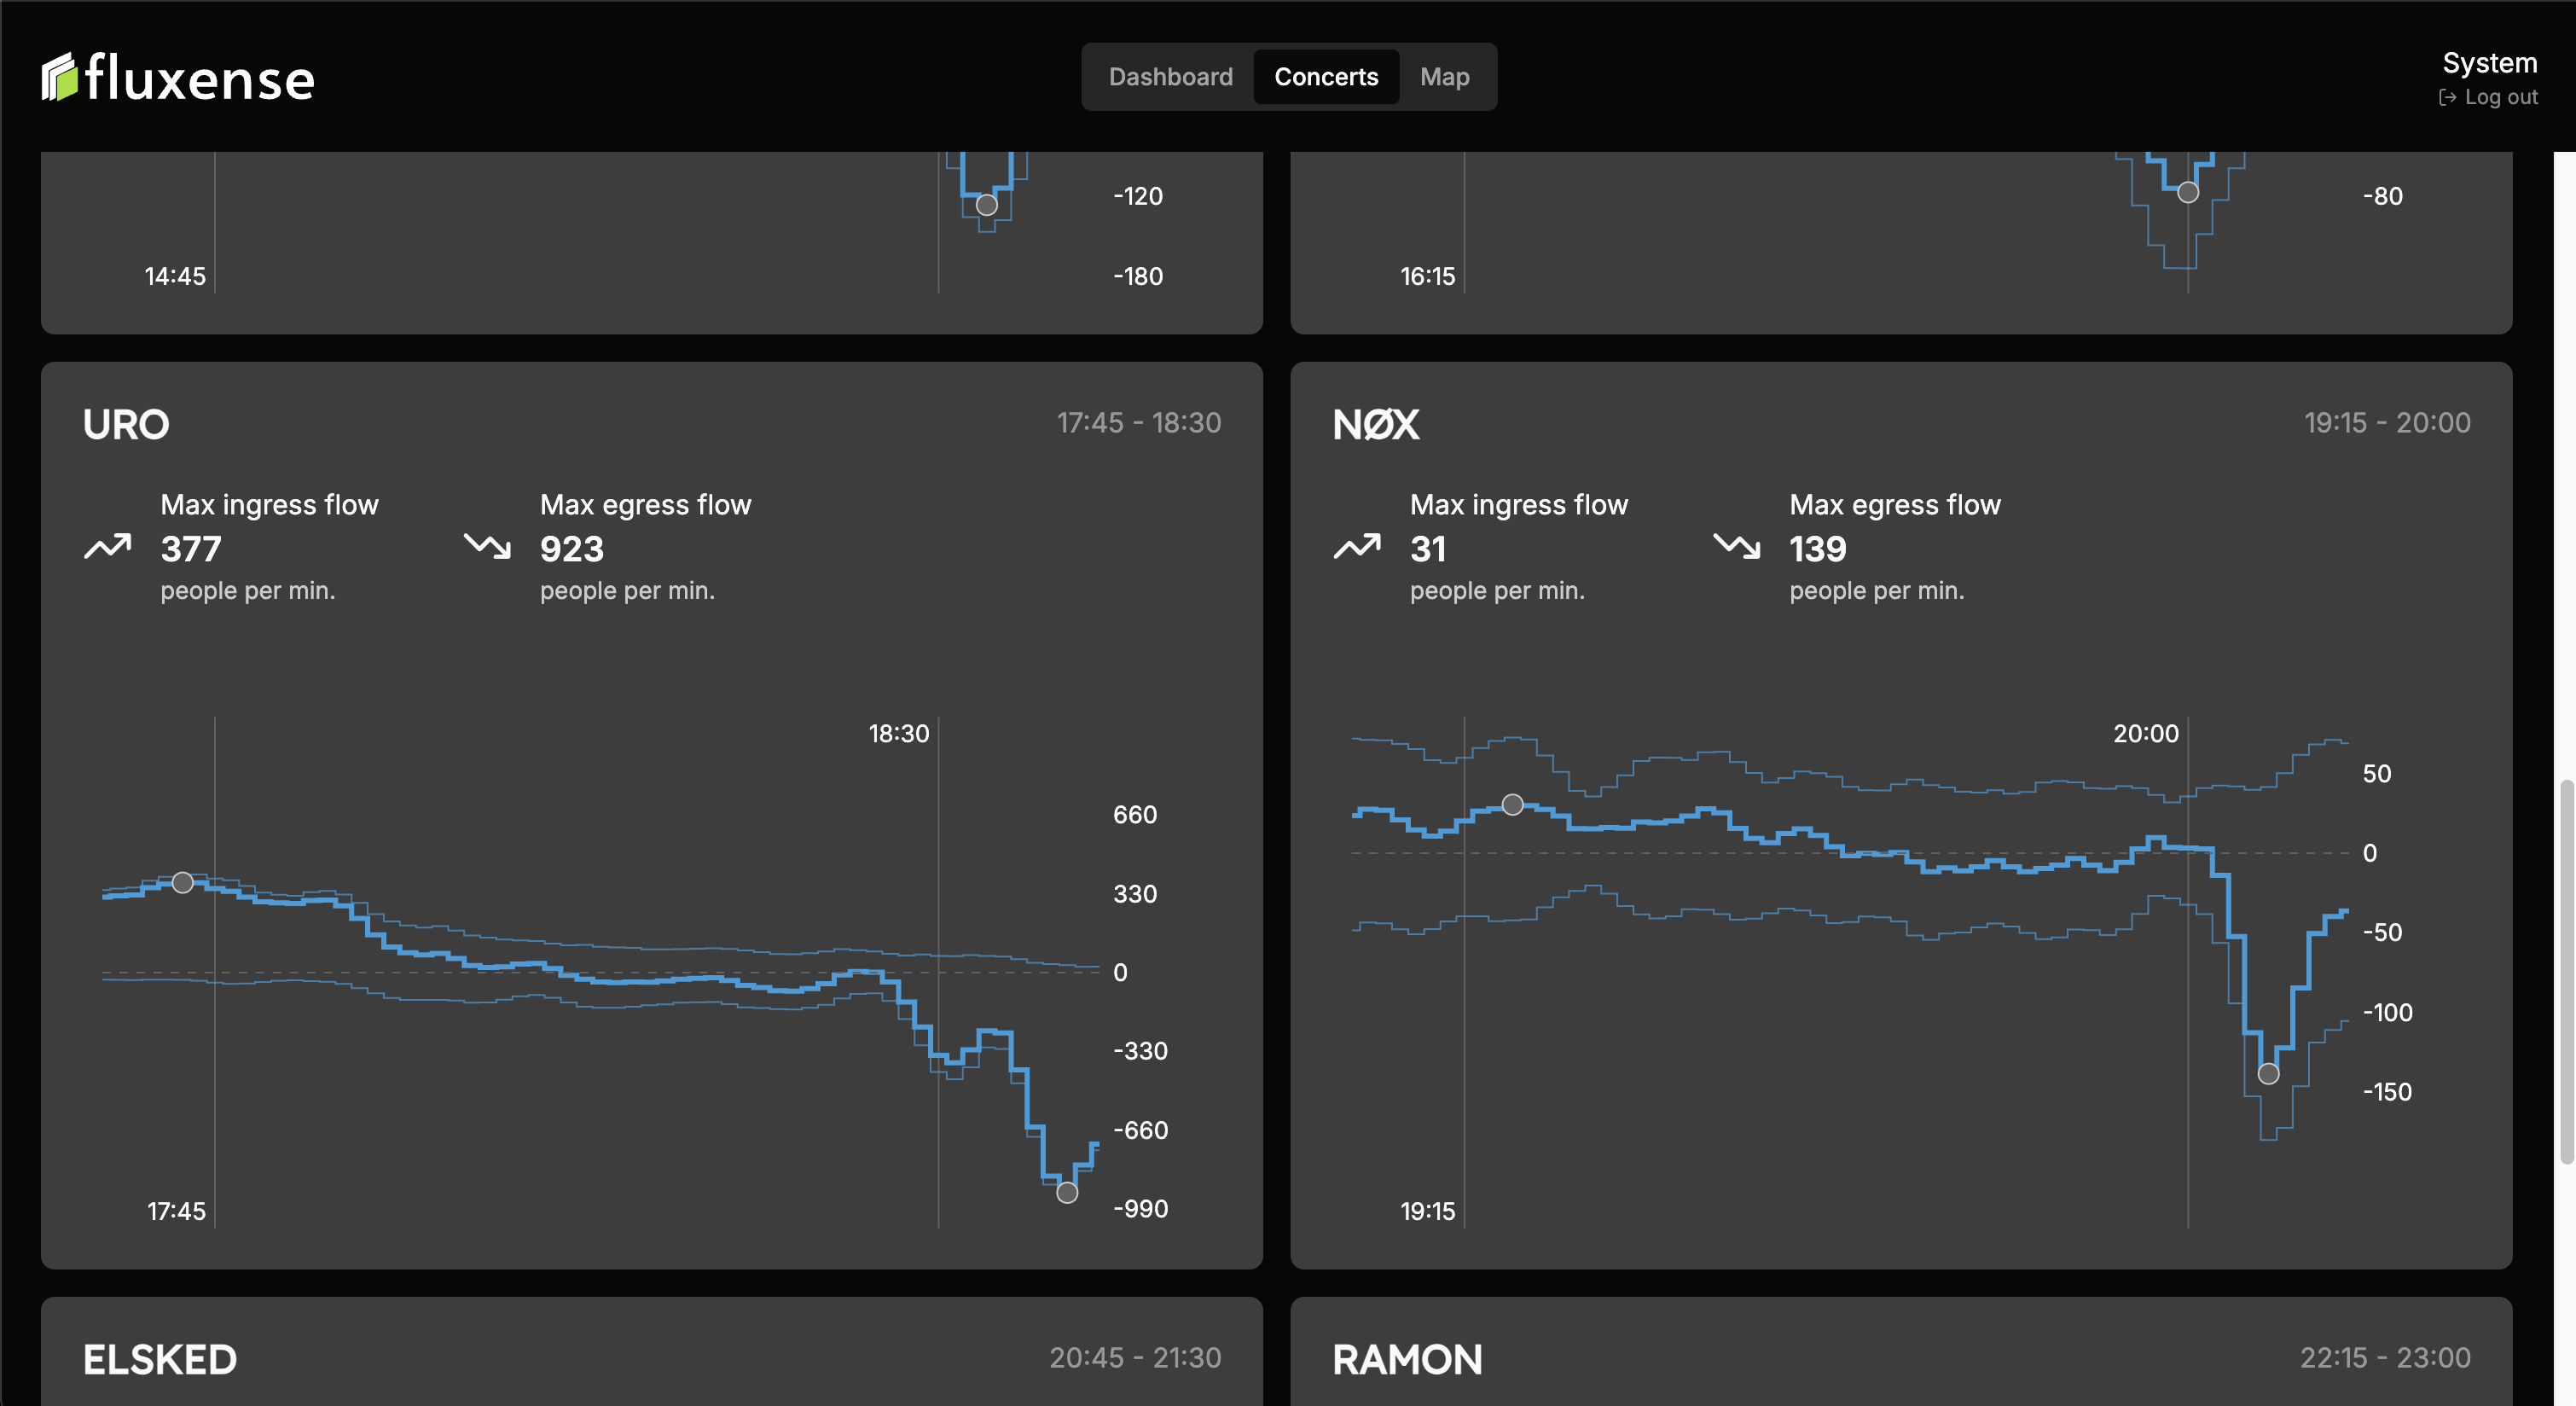
\includegraphics[width=\textwidth]{Pictures/Misc/Frontend/flow_concerts.png}
  \caption{The 'Concerts' view, with a breakdown of the flow rate data for individual concerts scheduled on the selected day. Each concert card shows the flow during the concert period and highlights the maximum observed ingress and egress flow rates in people per minute.}
  \label{fig:showcase:concerts}

\end{figure}

\begin{figure}[H]
  \centering
  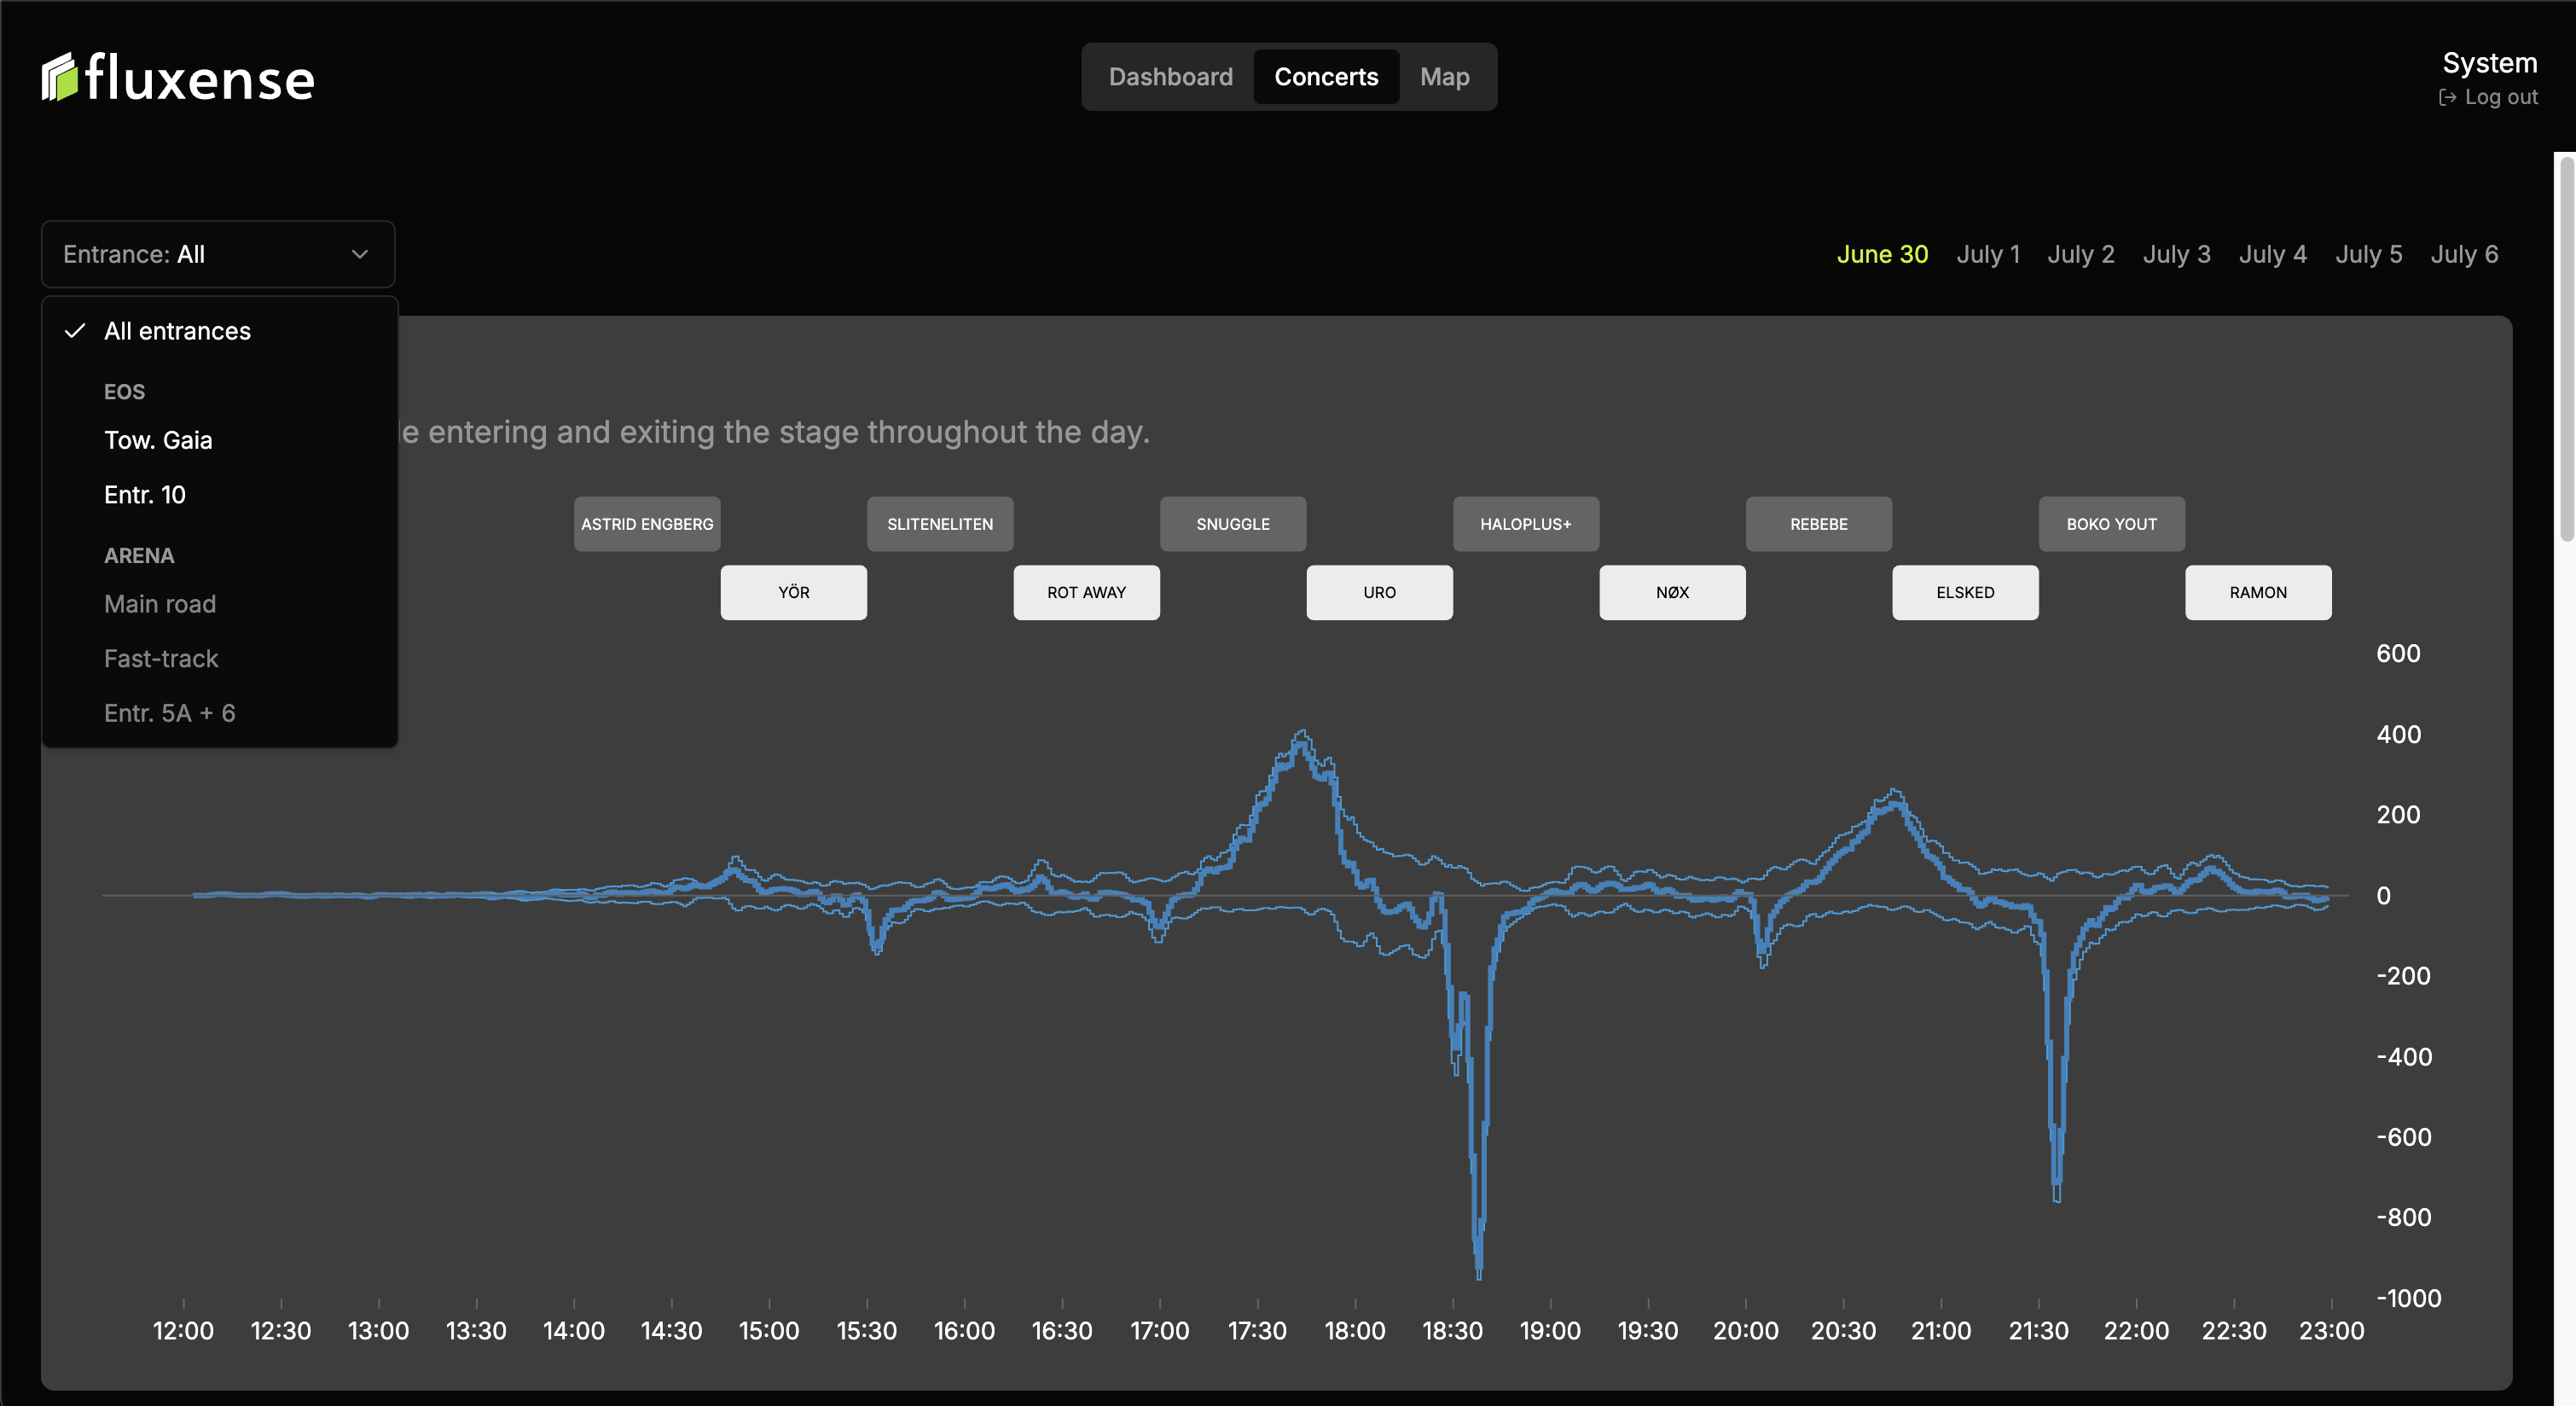
\includegraphics[width=\textwidth]{Pictures/Misc/Frontend/entrance_filter.png}
  \caption{The filtering controls available in the application, refined based on user requirements identified during feedback sessions. Users can select the date and filter the displayed data by specific entrances or view aggregated data for all entrances at a stage.}
  \label{fig:showcase:filter}
\end{figure}

\begin{figure}[H]
  \centering
  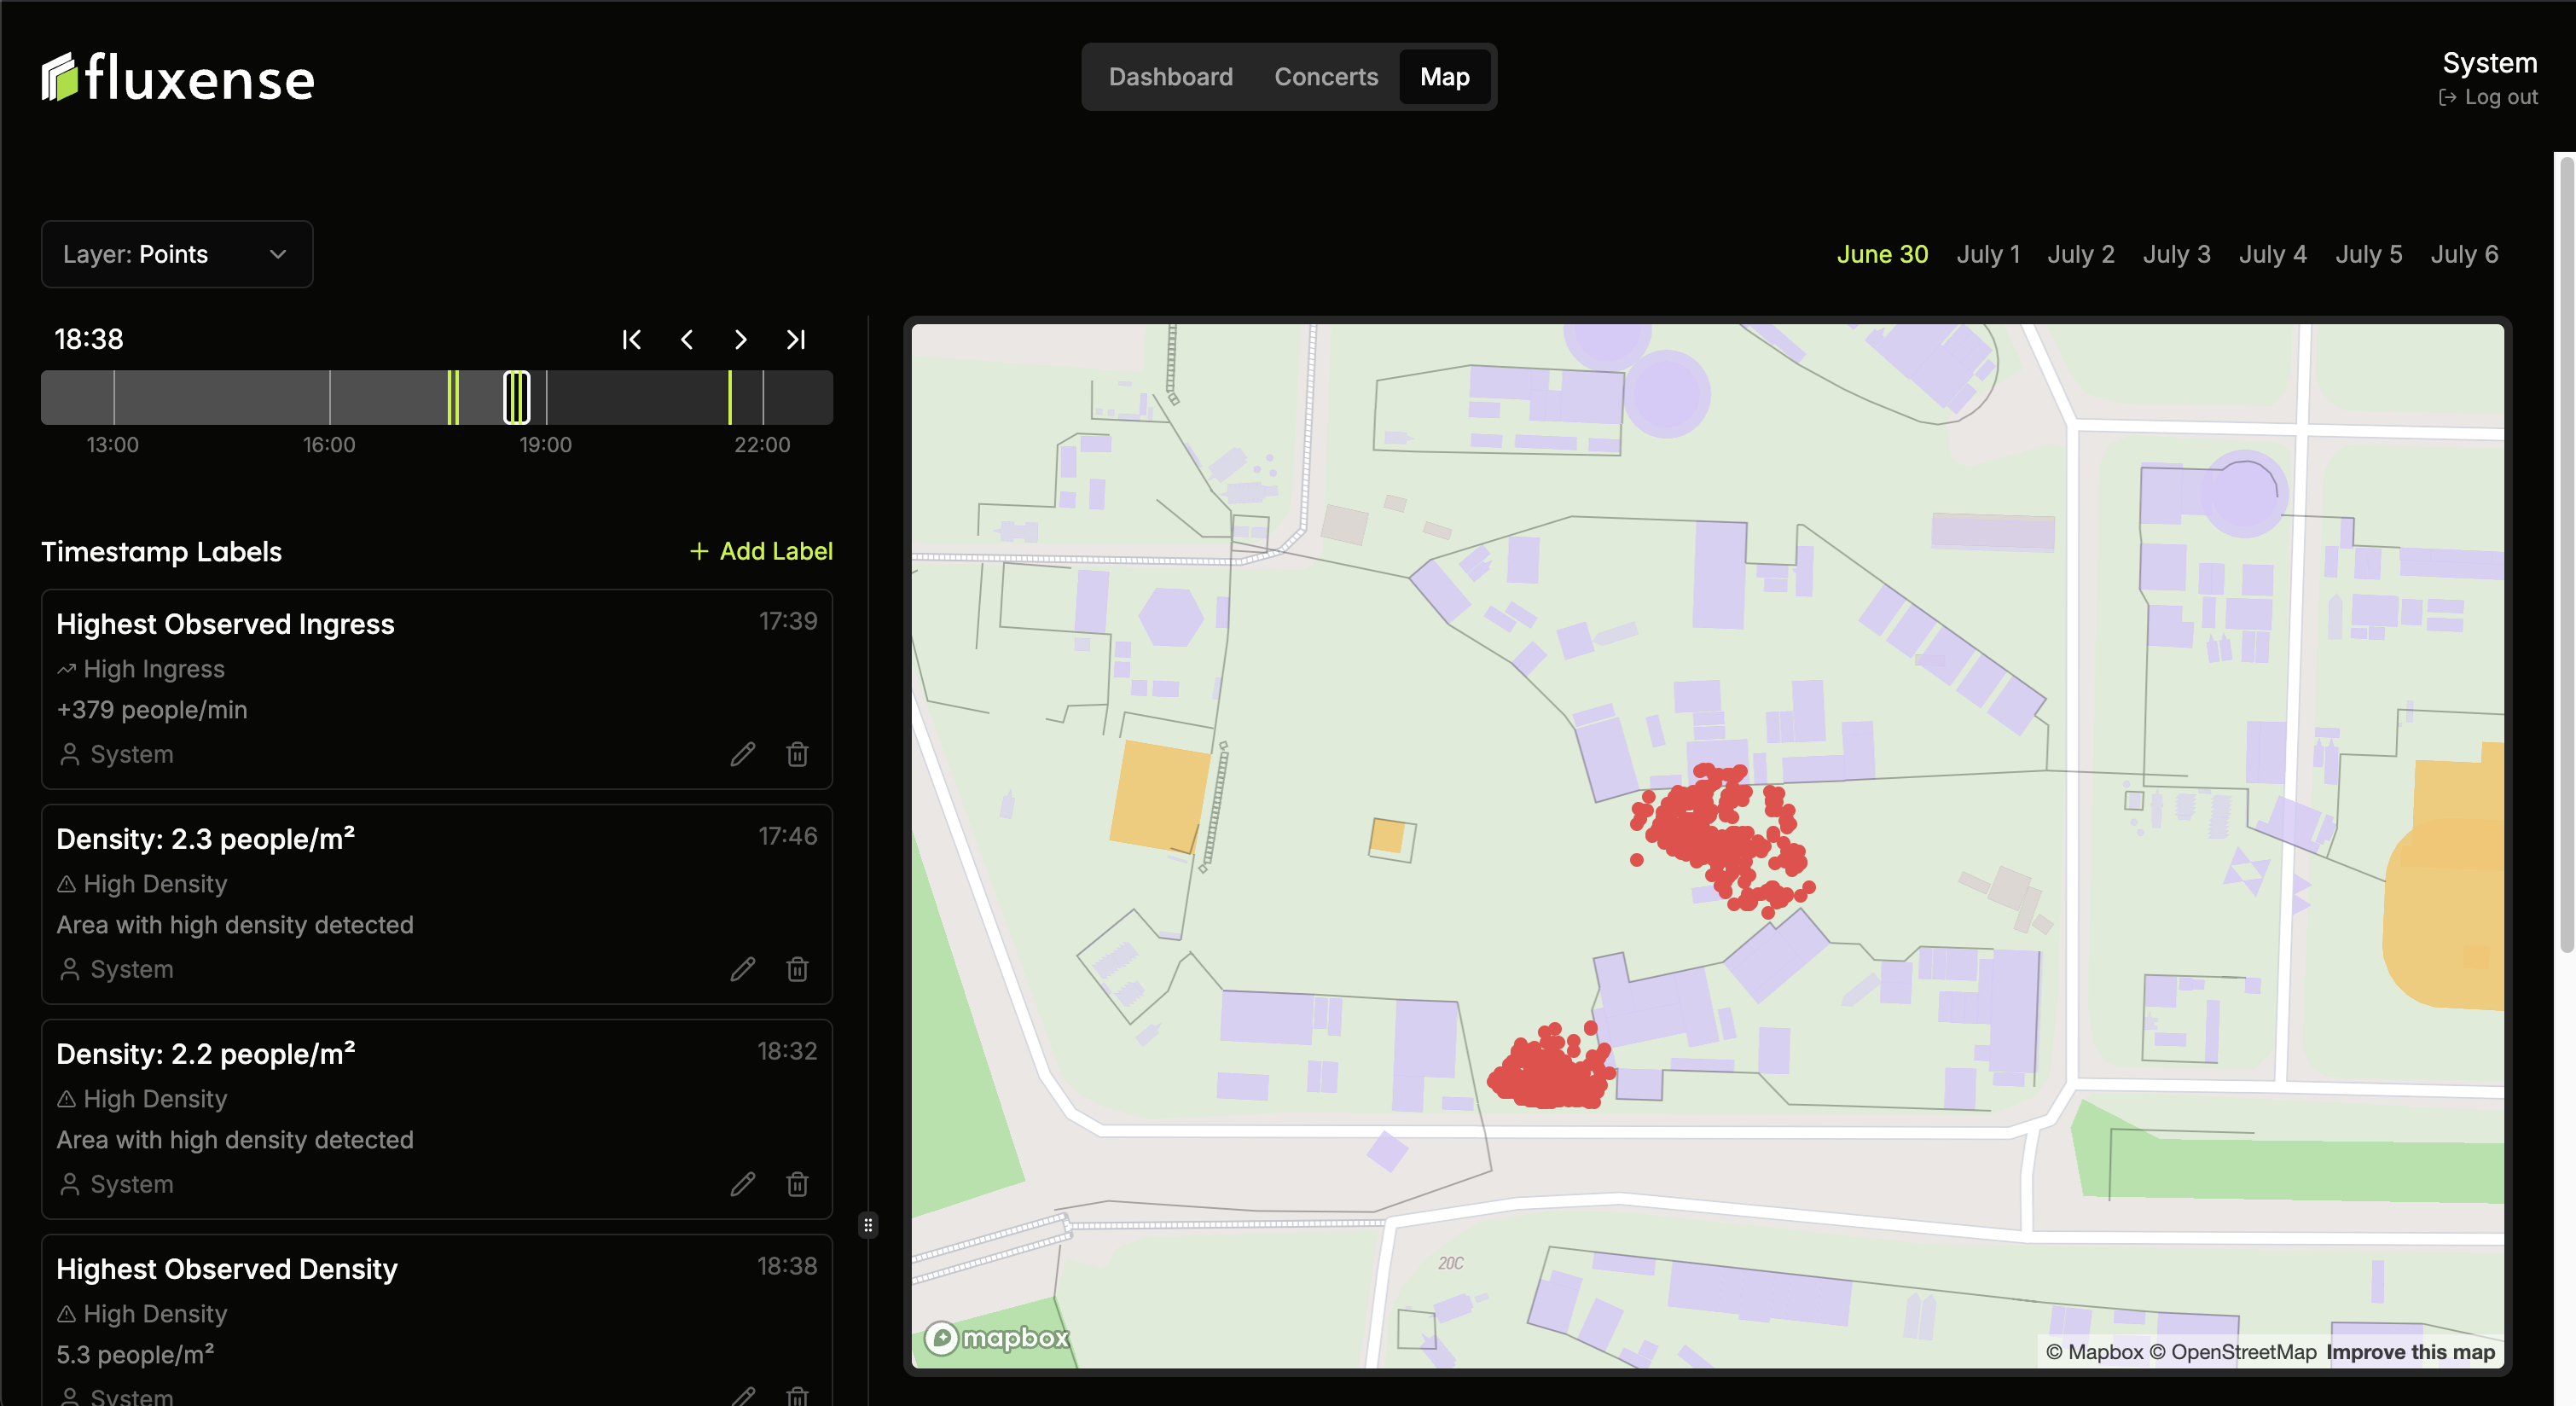
\includegraphics[width=\textwidth]{Pictures/Misc/Frontend/map_points.png}
  \caption{The 'Map' view interface elements. This includes an interactive timeline slider for navigating through the day, the 'Timestamp Labels' feature for adding notes, and the map displaying positional data for the selected time. The map layer itself can be configured to show individual detections as scatter points, as seen here.}
  \label{fig:showcase:map-scatter}

\end{figure}

\begin{figure}[H]
  \centering
  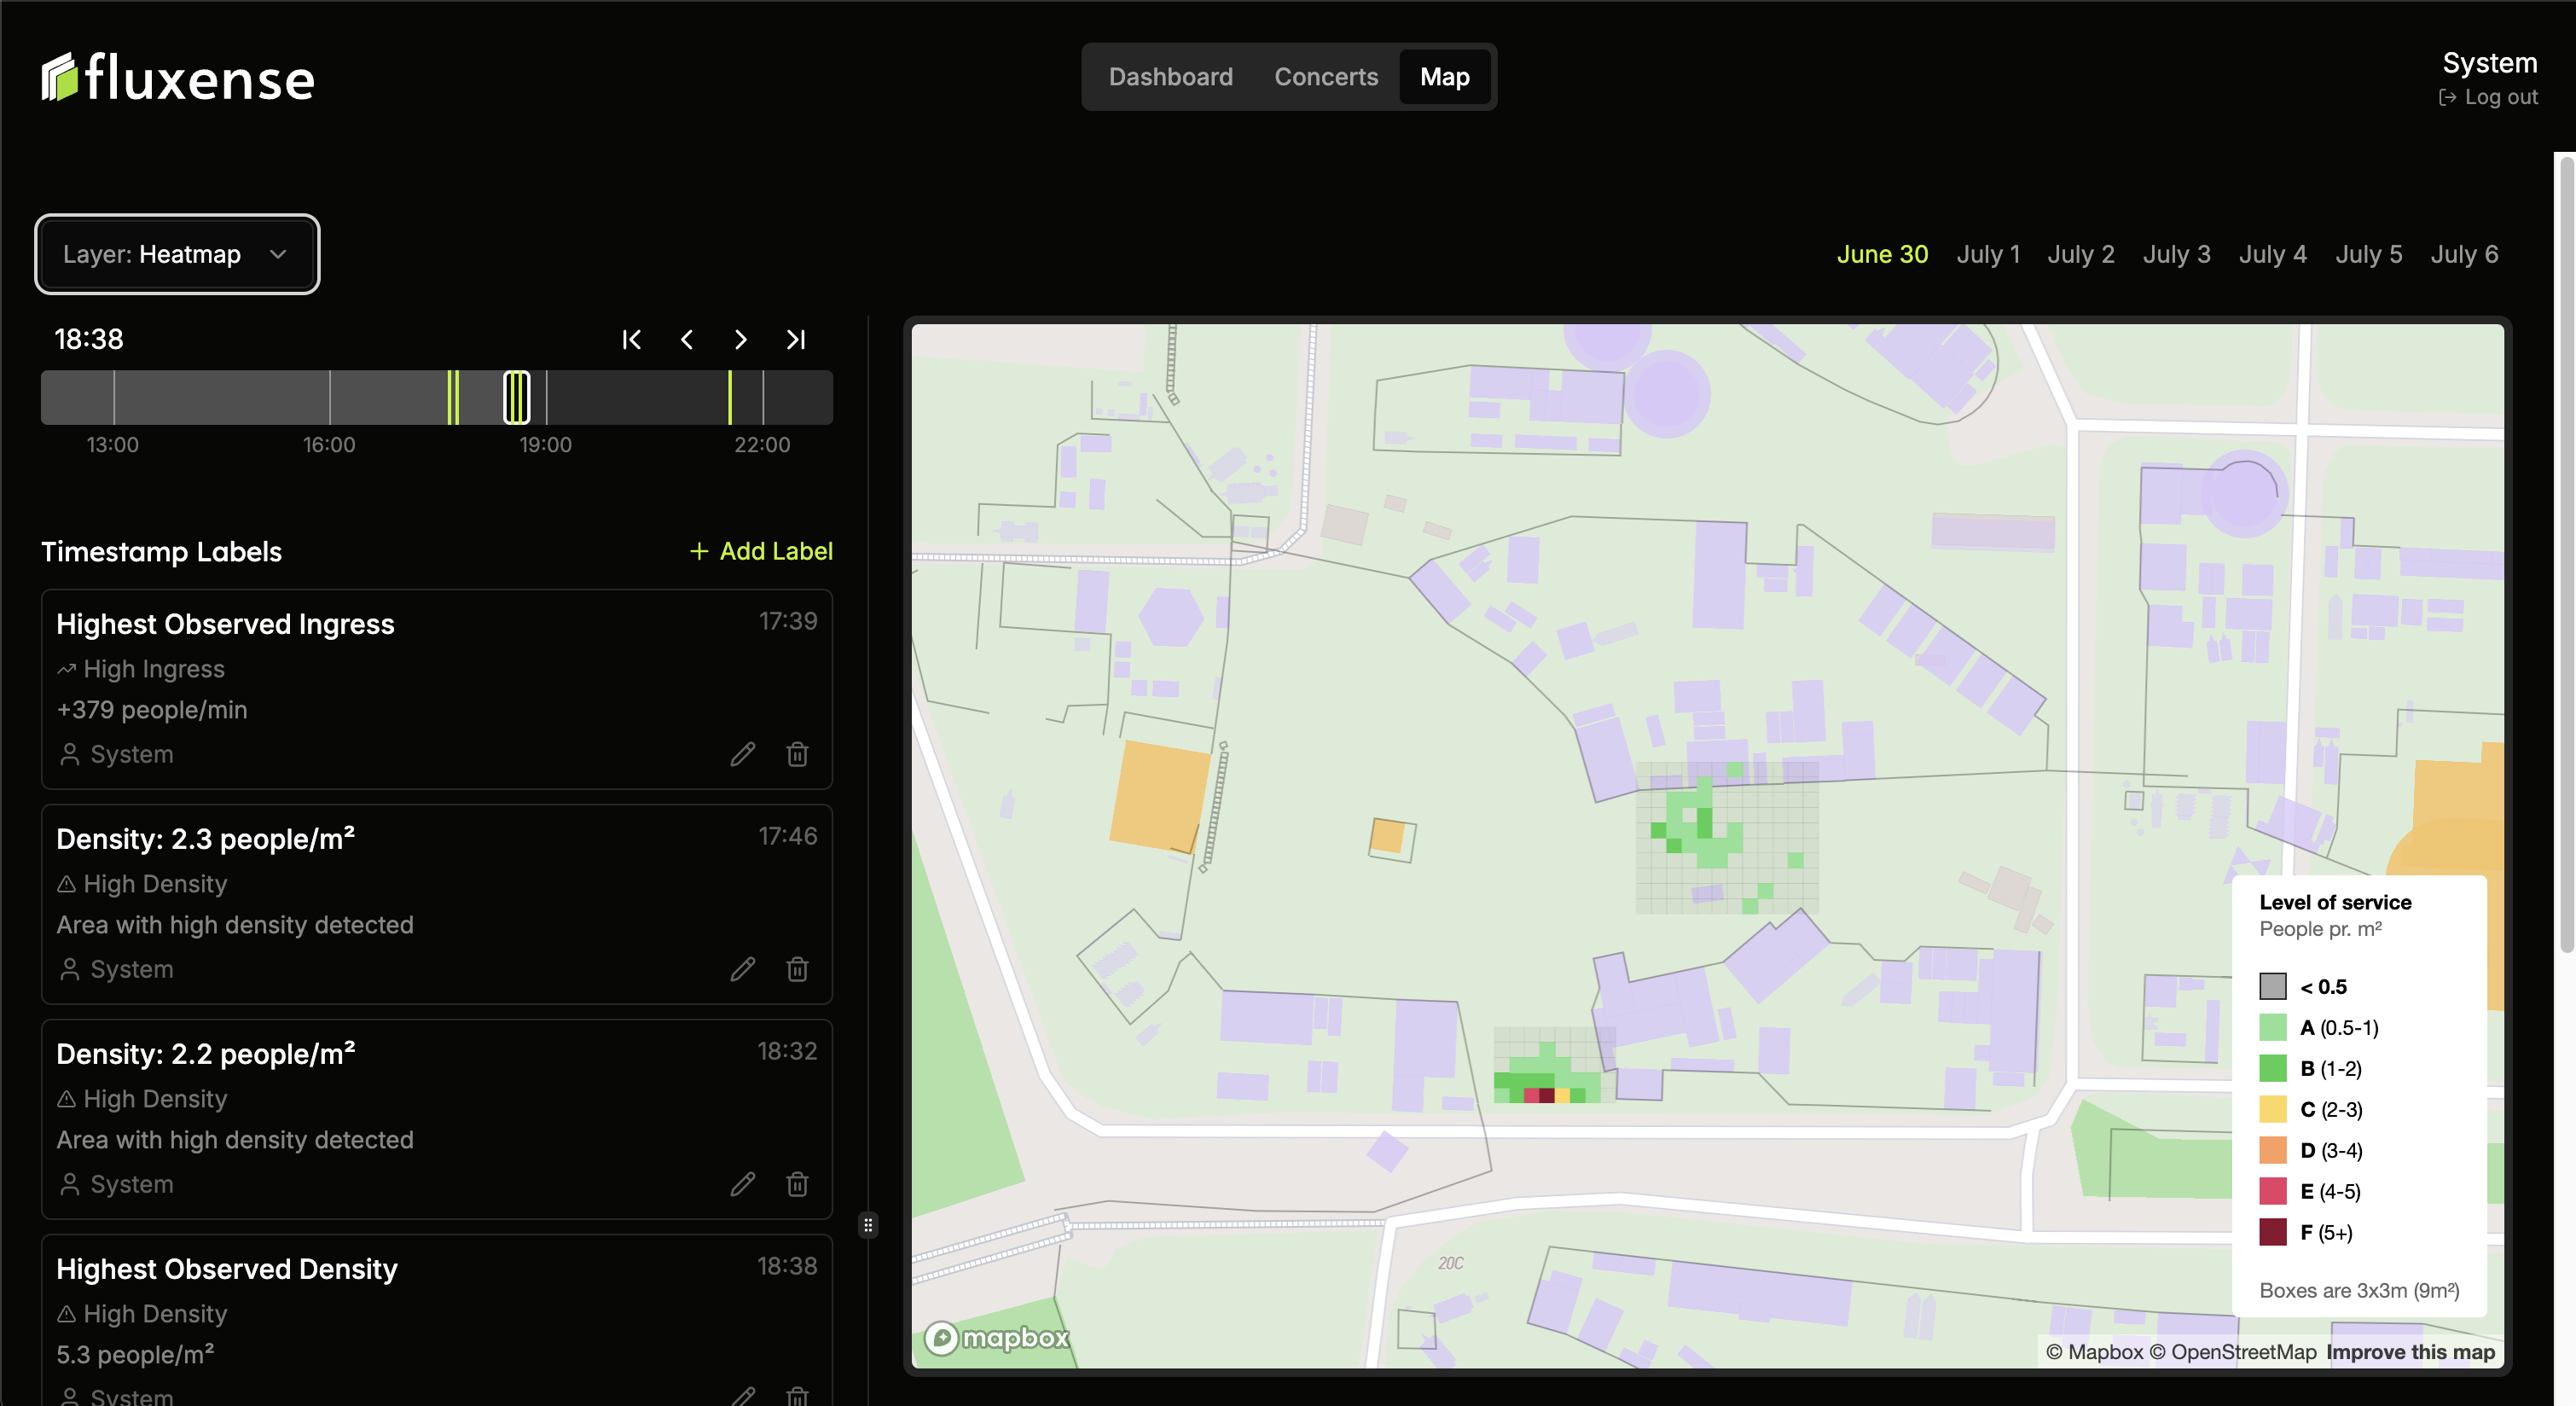
\includegraphics[width=\textwidth]{Pictures/Misc/Frontend/map_density.png}
  \caption{The 'Map' view displaying the 'Heatmap' layer. Crowd density is visualized using colored 3x3 meter grid cells. Following feedback, the color scale corresponds to Roskilde Festival's internal Levels of Service (LoS) scale (A-F), indicating people per square meter (people/m\textsuperscript{2}) to align with their existing practices.}
  \label{fig:showcase:map-density}

\end{figure}

\begin{figure}[H]
  \centering
  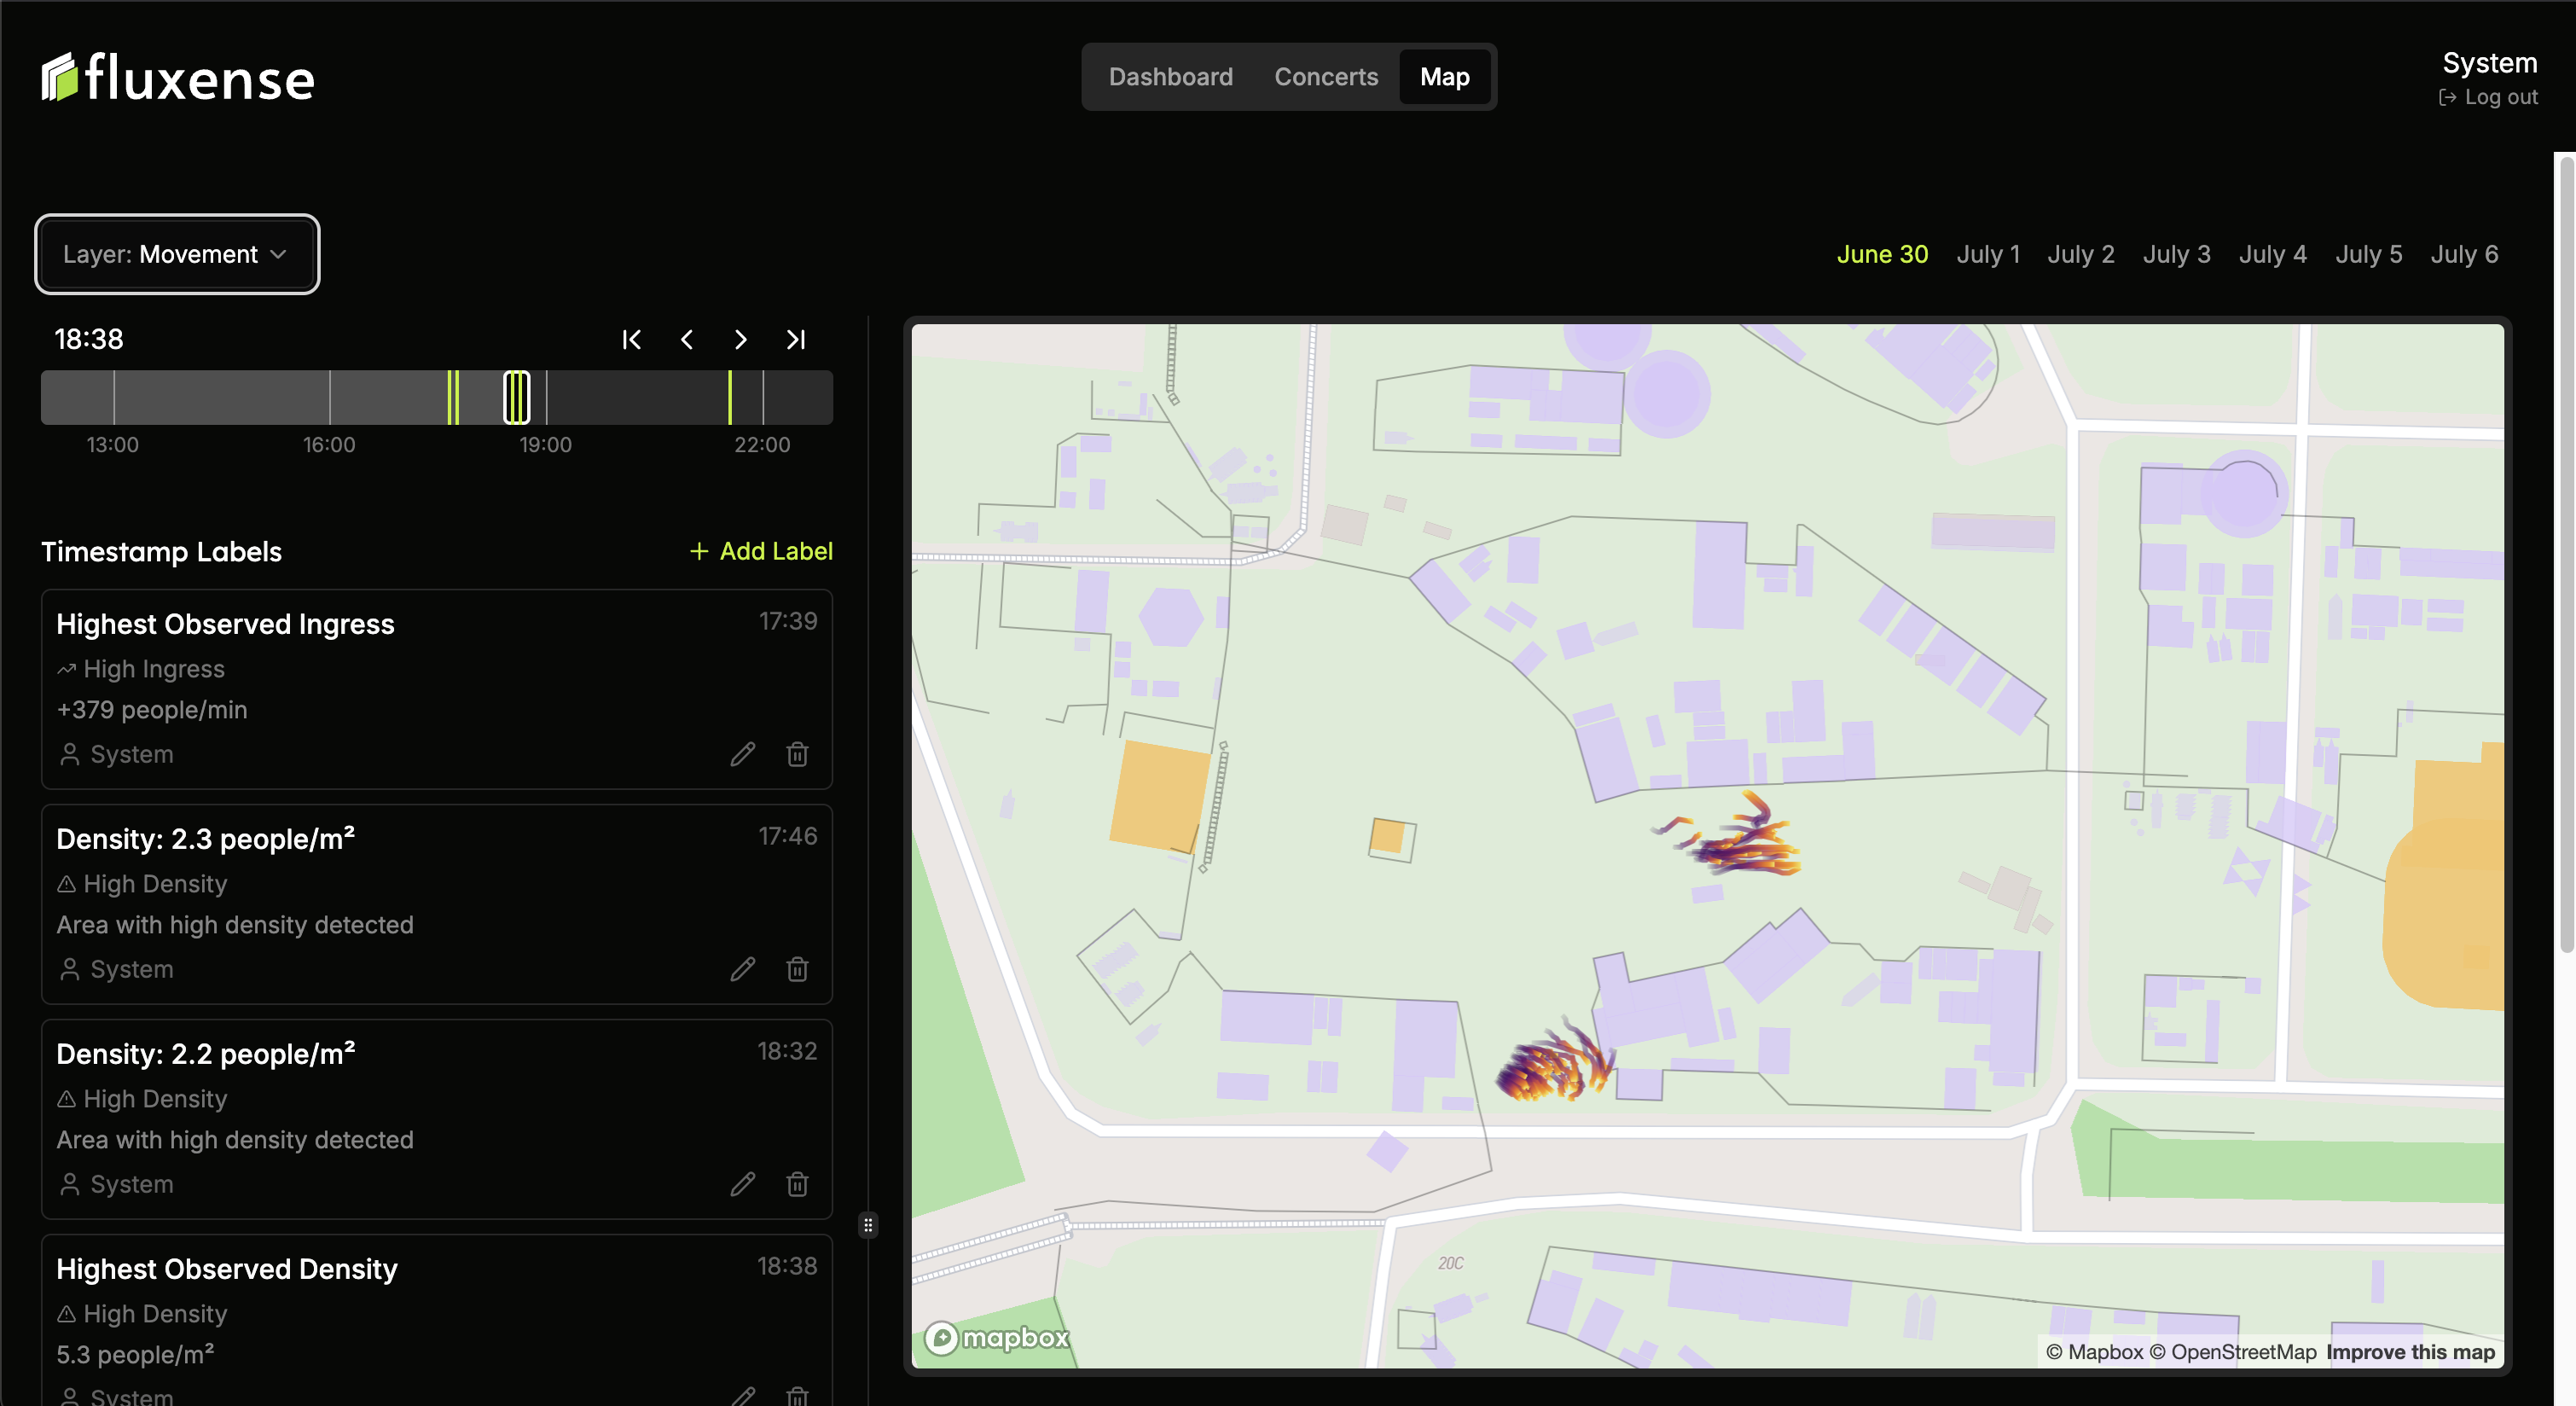
\includegraphics[width=\textwidth]{Pictures/Misc/Frontend/map_movement.png}
  \caption{The 'Map' view displaying the 'Movement' layer. Developed in response to feedback requesting visualization of movement patterns, it shows the trajectories of tracked individuals as lines on the map, with color gradients indicating the direction of movement, helping to visualize flow and origin-destination patterns.}
  \label{fig:showcase:map-movement}

\end{figure}


\begin{figure}[H]
  \centering
  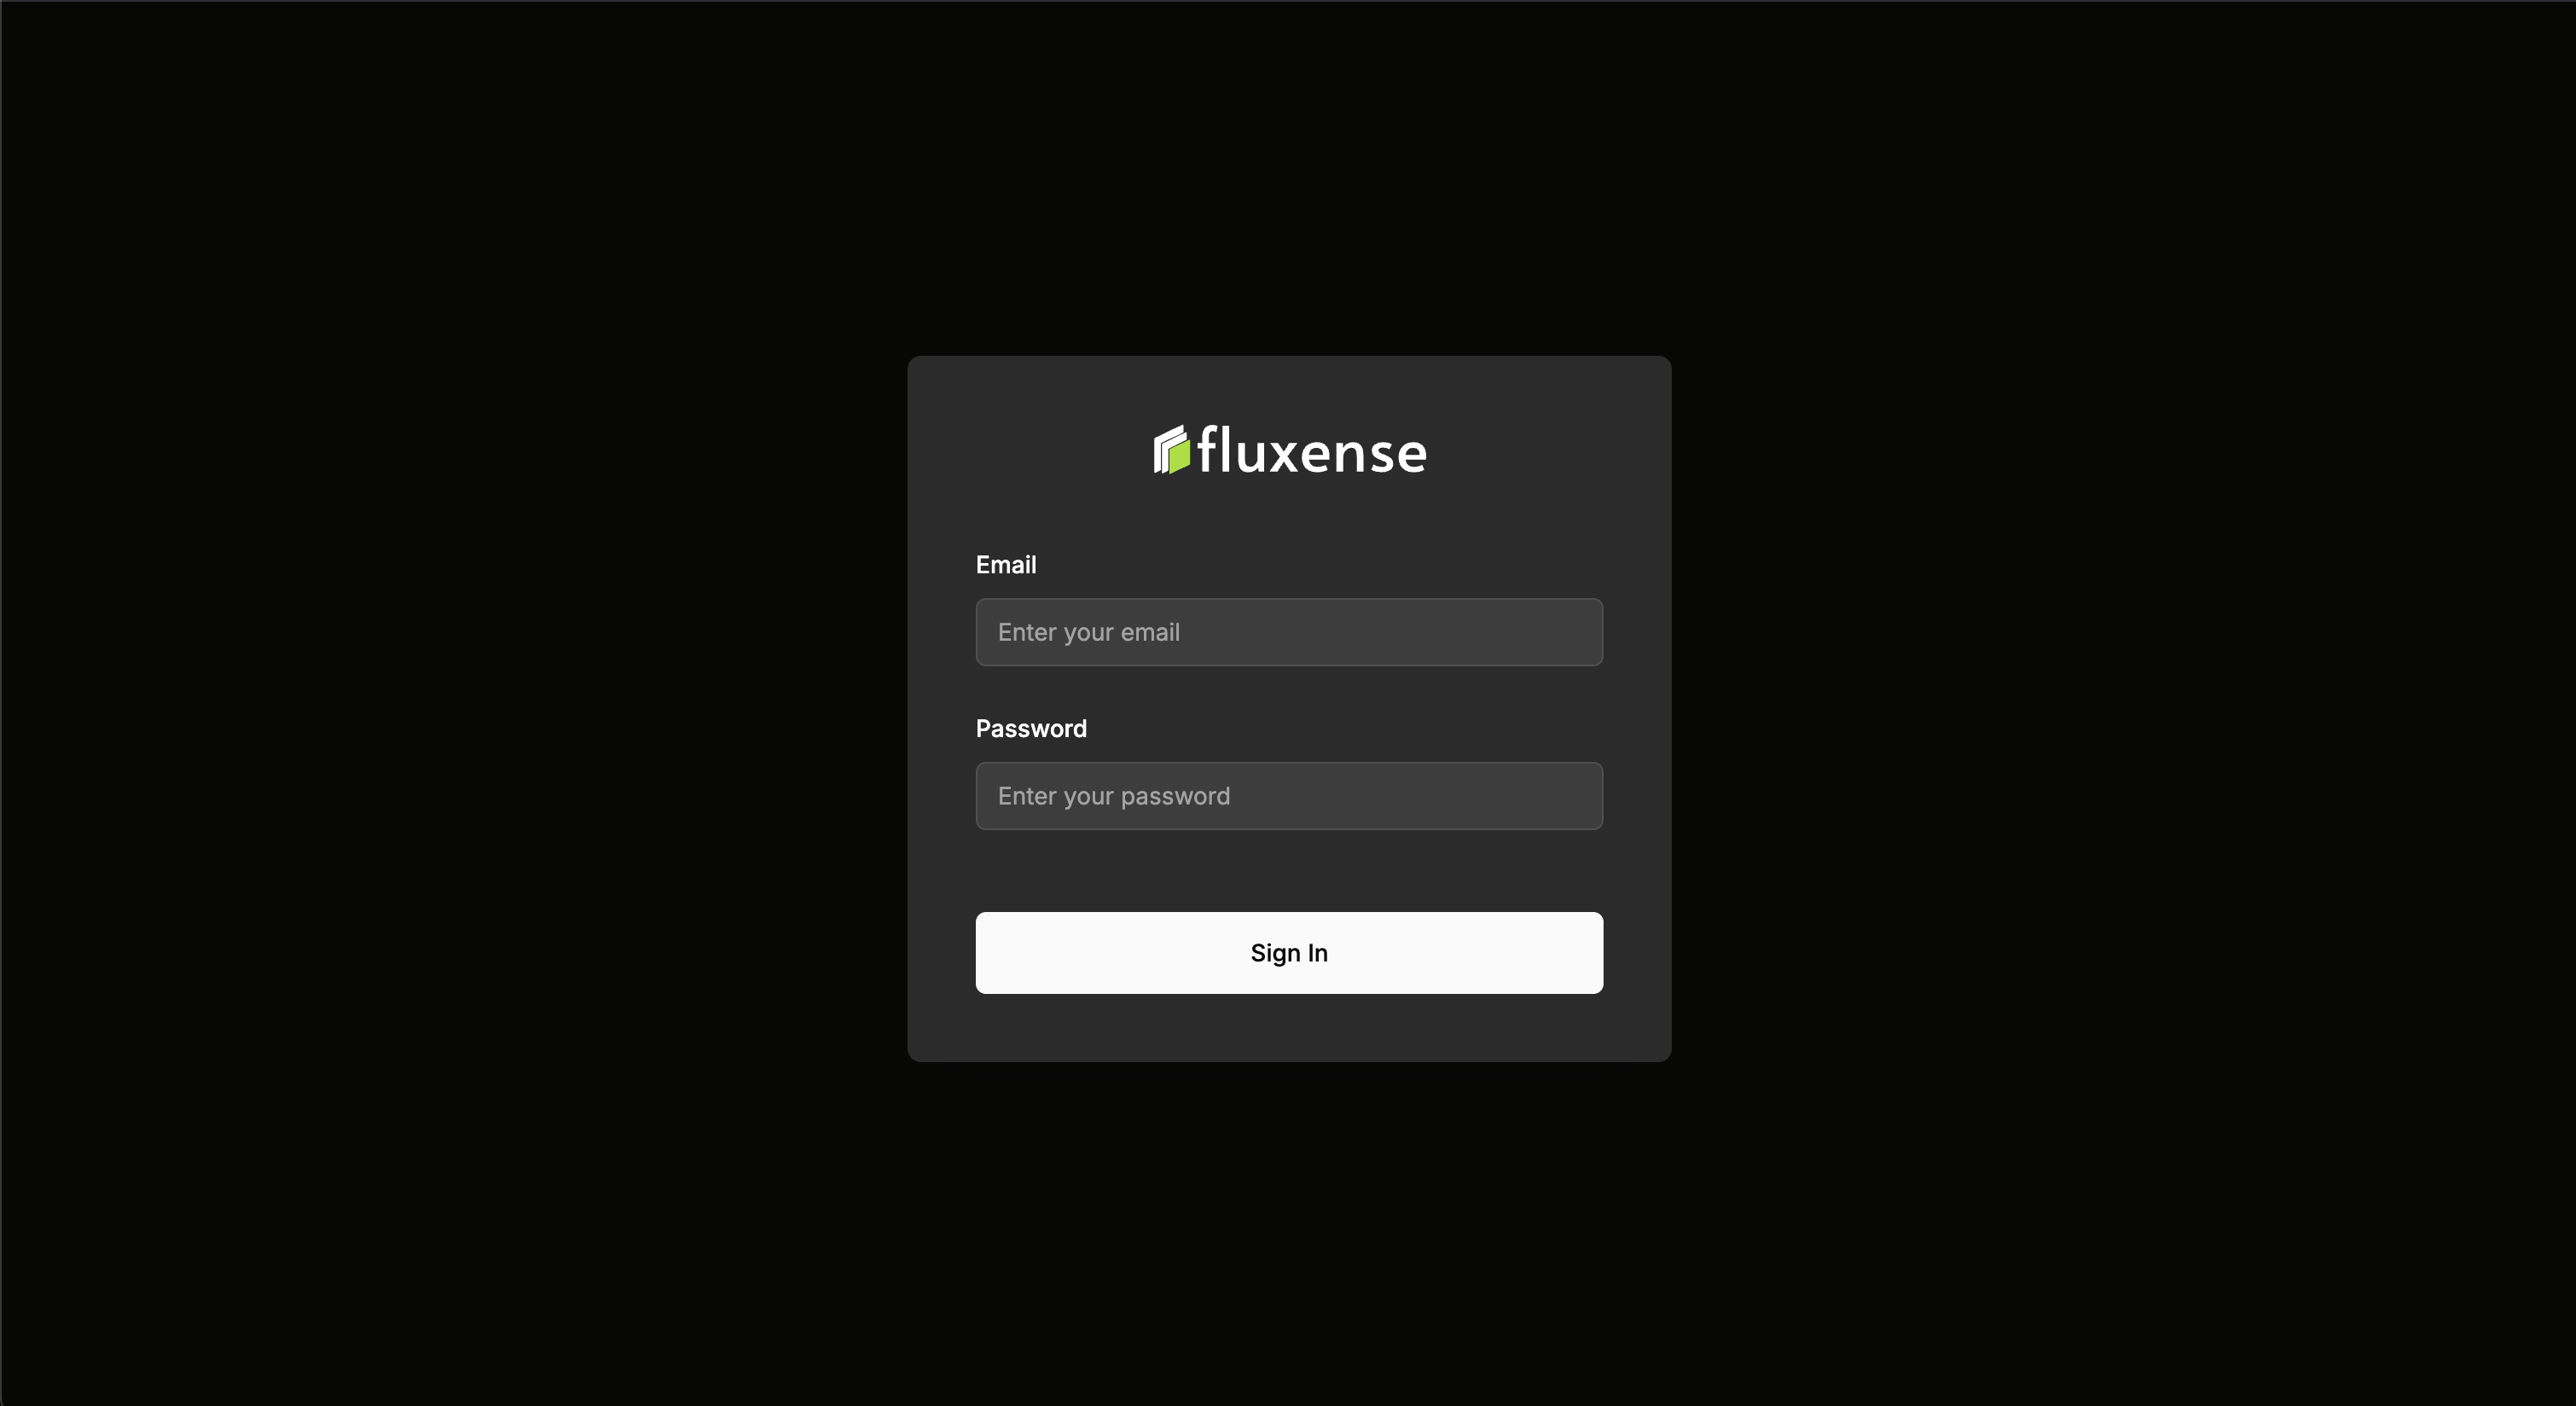
\includegraphics[width=\textwidth]{Pictures/Misc/Frontend/login.png}
  \caption{The application login screen, ensuring secure access to the crowd analysis data.}
  \label{fig:showcase:login}

\end{figure}



\section{Technical performance evaluation}


\section{Business value}
\label{sec:business-value}

In order to evaluate the business value of the developed product, a workshop was held with two key members of the Roskilde Festival safety team, Mads Therkilden (Safety Lead) and Niels Laustsen (Program Safety Team Lead). The workshop began with a demonstration of the results of the project, where participants were shown the final product and its capabilities, subsequently providing login credentials to access the application themselves. The remainder was structured around a series of scenarios that the safety team might encounter during the planning of the festival. The scenarios were designed in order to test whether the developed product could provide a concrete value in certain situations. The scenarios were as follows:

\begin{enumerate}
  \item \textbf{Scenario 1:} Entrance 10 is a primary access point for the Eos stage, especially crucial during the first days. Let's assume festival-goer feedback from Roskilde Festival (RF) 2024 suggested this entrance felt congested at times. The safety team needs to assess if the current width is adequate or requires modification for RF 2025 to handle peak demand safely.
  \item \textbf{Scenario 2:} Your colleague from Food \& Beverage (F\&B) proposes moving the popular Cava Bar to the main corridor leading to/from Entrance 10 to capture more foot traffic. The safety team is concerned because they believe this corridor already experiences some congestion during peak times. Adding a bar with likely queues could create unsafe scenarios. The task is to explain to the F\&B colleague these concerns and justify recommending against the relocation.
  \item \textbf{Scenario 3:} A colleague questions the back-to-back scheduling of the Eos and Gaia stages during the first days, concerned that it could lead to congestion between the stages. How can you determine and communicate whether or not the scheduling strategy was operationally sound?
\end{enumerate}

After presenting each scenario, the participants were requested to discuss how they would approach the scenario given their current workflows. Once they reached an agreement, they were asked to use the application to aid in solving the same scenario. After each the scenario, the participants were presented with a series of questions, aimed at quantitatively evaluating the business value of the product. The results of this evaluation can be found in (Appendix x). The questions were as follows:

\begin{enumerate}
  \item Overall, compared to your current process, how valuable do you perceive the approach using this tool to be for this specific task? (\textit{Scale 1-5: Not at all Valuable to Extremely Valuable})
  \item How do you think using this tool might impact the time or effort required for this task compared to your current methods? (\textit{Scale 1-5: Much More Effort to Much Less Effort})
  \item Compared to your current process, how might using the tool affect your confidence in the outcome related to this task? (\textit{Scale 1-5: Much Less Confident to Much More Confident})
\end{enumerate}

The workshop effectively demonstrated the product's value by applying it to realistic situations faced by the safety team. Analysis of the discussions and feedback for each scenario reveals how the tool addresses the specific business objectives defined in Section \ref{sec:objectives}, often by providing objective data lacking in current workflows.

The first scenario, assessing Entrance 10, highlighted the contrast between current subjective methods and the tool's objective data, primarily demonstrating its ability to create reliable documentation, as defined in Objective 3. Assessing such an issue in their current workflows is challenging, as it heavily depends on the availability of relevant CCTV footage, which is not guaranteed. Assuming footage exists, the team would need to manually search through it, and make subjective density estimates based on the Levels of Service model presented in Figure \ref{fig:fruin}. Given access to the application, the team could immediately find the historical density data for the specific entrance, identify the peak moments (e.g., a brief 5.3 people/m\textsuperscript{2} spike), and observe a dissipation after a few minutes. This aided the team in concluding that the short-lived peak was concerning enough to warrant a significant change in the existing infrastructure. The scenario demonstrated the tool's ability to provide objective, easily accessible documentation, replacing intuition based decisions and time-consuming searches through incomplete data sources, which was reflected in high ratings for value (4/5) and effort reduction (5/5).

The second scenario, concerning the Cava Bar relocation, clearly contrasted current communication efforts with the tool's visual evidence, impacting internal communication (Objective 1) and safety planning (Objective 2). Assuming the team has access to the information gathered in the first scenario, the current workflow relies heavily on verbal arguments to justify safety concerns to other departments, such as Food \& Beverage. If further justification is needed, Mads Therkildsen explained he would manually create visuals, for instance using PowerPoint, to illustrate theoretical concerns like cross-flow or queue formation -- a time-consuming process requiring skills outside their core competencies. Given the application, the team can instantly collect objective visual evidence by taking screenshots of density heatmaps or movement flow patterns. This easily accessible, objective visual evidence significantly strengthens their planning recommendations and makes communication with colleagues more efficient, as reflected in the 5/5 rating for effort reduction.

Finally, the third scenario, involving back-to-back concert scheduling between Eos and Gaia, demonstrated the tool's ability to replace estimation with concrete data, enhancing safety planning (Objective 2) and creating reliable documentation (Objective 3). The current workflow bases planning on estimations: calculating required pathway widths using the theoretical maximum capacity of a stage (e.g., 8000 for Eos) and applying standard formulas based on pathway width. This method relies on assumptions about crowd size, which is currently impossible to accurately calculate, as well as expected behavior based on concert assessments, as discussed in Section \ref{existing-frameworks}. The safety team subsequently used the application to identify actual peak attendance (closer to 10,000) and, more importantly, the actual peak flow rate through the specific connecting pathway (around 350 people/minute). This information allowed the team to rapidly assess that the existing infrastructure was sufficient to support maximum capacity. This scenario generally received lower ratings than the previous two, as estimates are already aimed to accommodate worst-case scenarios. However, the shift from estimation-based planning to data-validated planning helps increase confidence in previous decisions, as reflected in the 4/5 rating.

Following the three scenarios, the participants were asked to reflect on the overall value of the product, as well as emerging values that were not initially anticipated. Generally speaking, the feedback was overwhelmingly positive, especially regarding improvements to internal and external communication. Niels Laustsen expressed a frustration with the current process of communicating safety requirements, and expressed that the product could likely save him around two days of work in the planning phase, just in this application. The team found the greatest potential emerging given more footage and data across the festival site. Mads Therkildsen expressed that the product could play an integral role in planning entrances around the Arena stage, which is a chronic concern for the safety team. Arena is located in the eastern corner of the festival site, contributing to a significant imbalance in the distribution of attendees. Several attempts have been made to address this issue, but Mads sees potential for the product to provide objective data to evaluate their effectiveness in distrusting festival-goers. Niels provided a similar example, where the product could be used to determine fencing layout in front of the Orange Stage. He directly refers to the Astroworld incident mentioned in the introduction (Section \ref{sec:background}), and expressed that the product could be used to determine ingress imbalance around the front pit area.

In conclusion, the workshop confirmed that the developed platform provides substantial business value by directly addressing the business objectives and improving upon current workflows. Its value was demonstrated in enhancing safety planning with data replacing estimations, improving internal communication with accessible, objective visual evidence, and documenting for analysis, justification, and knowledge retention within Roskilde Festival's safety team.